% =====================================================================
%  MẪU BÁO CÁO TIỂU LUẬN HỌC PHẦN HỌC MÁY - Nguyễn Tuấn Anh
%  ---------------------------------------------------------------------
%  Biên dịch bằng XeLaTeX (hoặc LuaLaTeX), chạy 2 lần để cập nhật mục lục.
%  Trên Overleaf: Menu > Compiler > XeLaTeX.
%  Trên máy:      latexmk -xelatex "Mau bao cao mon Hoc may.tex"
%
%  Cách dùng mẫu:
%   1. Sửa THÔNG TIN BÁO CÁO ở mục (A) bên dưới.
%   2. Viết nội dung vào các chương; xóa các đoạn \huongdan{...} khi hoàn thành.
%   3. Đặt hình vào thư mục images/ và thay các khung \khunghinh{...}
%      bằng \includegraphics[width=...]{ten_hinh.png}.
% =====================================================================
\documentclass[12pt,a4paper,oneside]{report}

% Cỡ chữ thân bài 13pt (theo quy định trình bày của bộ môn)
\makeatletter
\renewcommand\normalsize{%
  \@setfontsize\normalsize{13pt}{15.6pt}%
  \abovedisplayskip 12pt plus3pt minus7pt
  \belowdisplayskip \abovedisplayskip
  \abovedisplayshortskip 0pt plus3pt
  \belowdisplayshortskip 6.5pt plus3.5pt minus3pt}
\normalsize
\makeatother

% =====================================================================
%  (A) THÔNG TIN BÁO CÁO - SINH VIÊN SỬA TẠI ĐÂY
% =====================================================================
\newcommand{\truong}{TRƯỜNG ĐẠI HỌC CÔNG NGHỆ THÔNG TIN VÀ TRUYỀN THÔNG}
\newcommand{\khoa}{KHOA CÔNG NGHỆ THÔNG TIN}
\newcommand{\loaibaocao}{BÁO CÁO TIỂU LUẬN}
\newcommand{\hocphan}{Học máy}
\newcommand{\lophocphan}{KHMT K22}
\newcommand{\hocky}{Học kỳ 1, năm học 2026--2027}
\newcommand{\tendetai}{SO SÁNH CÁC THUẬT TOÁN HỌC MÁY TRUYỀN THỐNG TRONG DỰ ĐOÁN TƯƠNG TÁC THUỐC DỰA TRÊN CẤU TRÚC HÓA HỌC}
\newcommand{\tenbaitoan}{dự đoán tương tác thuốc} % dùng trong tên Chương 1 và 2
\newcommand{\giangvien}{Nguyễn Tuấn Anh}  % thêm học hàm/học vị nếu cần
\newcommand{\nhom}{Nhóm 18}
\newcommand{\svAten}{Sùng A Khua}
\newcommand{\svAma}{DTC235160020}
\newcommand{\svBten}{Hoàng Bảo Ngọc}
\newcommand{\svBma}{DTC235160033}
\newcommand{\diadiem}{Thái Nguyên}
\newcommand{\thoigian}{tháng 10 năm 2026}

% ---------------- Trang giấy & phông chữ ----------------
\usepackage[a4paper,left=3cm,right=2cm,top=2.5cm,bottom=2.5cm,
            headheight=16pt,headsep=0.8cm]{geometry}
\usepackage{fontspec}
\setmainfont{Times New Roman}
\IfFontExistsTF{Consolas}{\setmonofont{Consolas}[Scale=0.9]}{\setmonofont{Courier New}[Scale=0.9]} % Overleaf khong co Consolas
\usepackage[vietnamese]{babel}
\usepackage{setspace}
\setstretch{1.3}
\setlength{\parindent}{1cm}
\setlength{\parskip}{6pt}
\usepackage{indentfirst}

% ---------------- Gói hỗ trợ ----------------
\usepackage{amsmath,amssymb}
\usepackage{graphicx}
\graphicspath{{images/}}
\usepackage{float}
\usepackage{array,booktabs,tabularx,multirow}
\usepackage{xltabular}
\setlength{\emergencystretch}{3em}
\renewcommand{\arraystretch}{1.25}
\usepackage[table]{xcolor}
\usepackage{tikz}
\usetikzlibrary{positioning,arrows.meta,calc,fit,backgrounds}
\usepackage{caption}
\captionsetup{labelsep=period,labelfont=bf,font=normalsize,skip=6pt}
\captionsetup[table]{position=top}
\usepackage{titlesec}
\usepackage{titletoc}
\usepackage[nottoc]{tocbibind}   % đưa danh mục hình, bảng, TLTK vào mục lục
\usepackage{enumitem}
\setlist{nosep,leftmargin=1.6cm}
\usepackage{listings}
\usepackage{needspace}
\usepackage{cite}                % gộp trích dẫn: [4-6], [2, 4-6]
\usepackage{fancyhdr}
\usepackage[unicode]{hyperref}
\hypersetup{
  hidelinks,
  pdftitle={\tendetai},
  pdfauthor={\svAten, \svBten},
  pdfsubject={\loaibaocao\ học phần \hocphan},
  bookmarksnumbered=true,   % bookmark có số thứ tự chương, mục
  bookmarksopen=true,
  bookmarksopenlevel=0,
}
% Bookmark dạng "Chương 1. Tên chương", "1.1. Tên mục", "Phụ lục A. ..."
\newcommand{\bmchapname}{Chương}
\makeatletter
\newcommand*{\bm@prefix}{}
\let\bm@orig@writebookmark\Hy@writebookmark
\renewcommand*{\Hy@writebookmark}[5]{%
  \ifnum#4=0 \def\bm@prefix{\bmchapname\space}\else\def\bm@prefix{}\fi
  \bm@orig@writebookmark{#1}{#2}{#3}{#4}{#5}}
\renewcommand*{\Hy@numberline}[1]{\bm@prefix#1. }
\makeatother

% ---------------- Màu & định dạng mã nguồn ----------------
\definecolor{codebg}{RGB}{247,247,247}
\definecolor{codekw}{RGB}{0,51,153}
\definecolor{codecm}{RGB}{0,128,0}
\definecolor{codestr}{RGB}{163,21,21}
\definecolor{guide}{RGB}{110,110,110}
\lstdefinestyle{python}{
  language=Python,
  basicstyle=\ttfamily\small\setstretch{1.0},
  backgroundcolor=\color{codebg},
  keywordstyle=\color{codekw}\bfseries,
  commentstyle=\color{codecm}\itshape,
  stringstyle=\color{codestr},
  numbers=left, numberstyle=\tiny\color{guide}, numbersep=8pt,
  frame=single, rulecolor=\color{black!25},
  breaklines=true, showstringspaces=false, tabsize=4,
  xleftmargin=1.2em, framexleftmargin=1.2em,
  aboveskip=8pt, belowskip=8pt, columns=fullflexible, keepspaces=true,
}
\lstset{style=python}
\renewcommand{\lstlistingname}{Đoạn mã}
\renewcommand{\lstlistlistingname}{DANH MỤC ĐOẠN MÃ}

% ---------------- Tên gọi tiếng Việt ----------------
\addto\captionsvietnamese{%
  \renewcommand{\contentsname}{MỤC LỤC}%
  \renewcommand{\listfigurename}{DANH MỤC HÌNH ẢNH}%
  \renewcommand{\listtablename}{DANH MỤC BẢNG}%
  \renewcommand{\bibname}{TÀI LIỆU THAM KHẢO}%
  \renewcommand{\figurename}{Hình}%
  \renewcommand{\tablename}{Bảng}%
  \renewcommand{\chaptername}{Chương}%
  \renewcommand{\appendixname}{Phụ lục}%
}

% ---------------- Đầu trang & chân trang ----------------
\pagestyle{fancy}
\fancyhf{}
\fancyhead[L]{\small\itshape Báo cáo tiểu luận học phần \hocphan}
\fancyhead[R]{\small\itshape\nouppercase{\leftmark}}
\fancyfoot[C]{\thepage}
\renewcommand{\headrulewidth}{0.4pt}
\renewcommand{\chaptermark}[1]{\markboth{\chaptertitlename~\thechapter. #1}{}}
\fancypagestyle{plain}{\fancyhf{}\fancyfoot[C]{\thepage}\renewcommand{\headrulewidth}{0pt}}

% ---------------- Định dạng tiêu đề ----------------
% Chương: "CHƯƠNG 1" + tên chương in hoa - 14pt, đậm, căn giữa
\titleformat{\chapter}[display]
  {\filcenter\bfseries\fontsize{14}{18}\selectfont}
  {\MakeUppercase{\chaptertitlename}~\thechapter}{4pt}{\MakeUppercase}
\titlespacing*{\chapter}{0pt}{0pt}{18pt}
% Mục cấp 2: "1.1. Giới thiệu" - 14pt, đậm
\titleformat{\section}
  {\bfseries\fontsize{14}{18}\selectfont}{\thesection.}{0.5em}{}
\titlespacing*{\section}{0pt}{12pt}{6pt}
% Mục cấp 3: "1.1.1. Mục" - 13pt, đậm
\titleformat{\subsection}
  {\bfseries\fontsize{13}{17}\selectfont}{\thesubsection.}{0.5em}{}
\titlespacing*{\subsection}{0pt}{10pt}{6pt}
% Mục cấp 4: "1.1.1.1. Mục" - 13pt, đậm nghiêng
\setcounter{secnumdepth}{3}
\titleformat{\subsubsection}
  {\bfseries\itshape\fontsize{13}{17}\selectfont}{\thesubsubsection.}{0.5em}{}
\titlespacing*{\subsubsection}{0pt}{8pt}{4pt}

% ---------------- Mục lục & danh mục ----------------
\setcounter{tocdepth}{2}
\newcommand{\tocchapname}{Chương}
\titlecontents{chapter}[0pt]{\addvspace{6pt}\bfseries}
  {\tocchapname~\thecontentslabel.\enspace}{}{\titlerule*[0.6pc]{.}\contentspage}
\titlecontents{section}[1.5em]{}
  {\thecontentslabel.\enspace}{}{\titlerule*[0.6pc]{.}\contentspage}
\titlecontents{subsection}[3em]{}
  {\thecontentslabel.\enspace}{}{\titlerule*[0.6pc]{.}\contentspage}
\titlecontents{figure}[0pt]{}
  {\figurename~\thecontentslabel.\enspace}{}{\titlerule*[0.6pc]{.}\contentspage}
\titlecontents{table}[0pt]{}
  {\tablename~\thecontentslabel.\enspace}{}{\titlerule*[0.6pc]{.}\contentspage}

% ---------------- Lệnh tiện ích ----------------
% Chương không đánh số (Mở đầu, Kết luận...) vẫn có trong mục lục và đầu trang
\newcommand{\unnumberedchapter}[1]{%
  \chapter*{#1}\phantomsection\addcontentsline{toc}{chapter}{#1}\markboth{#1}{}}
% Ghi chú hướng dẫn (xóa khi viết xong)
\newcommand{\huongdan}[1]{{\color{guide}\itshape [Hướng dẫn: #1]}}
% Khung giữ chỗ cho hình: \khunghinh{rộng}{cao}{nội dung}
\newcommand{\khunghinh}[3]{%
  \begin{tikzpicture}
    \draw[dashed,thick,black!40,fill=black!3] (0,0) rectangle (#1,#2);
    \node[text width=0.8*#1,align=center,font=\itshape\color{guide}]
      at ($(0,0)!0.5!(#1,#2)$) {#3};
  \end{tikzpicture}}
% Dòng chấm để viết tay
% Ghi chú cần bổ sung (hiện màu đỏ, xóa khi đã điền)
\newcommand{\canbosung}[1]{{\color{red}[#1]}}
\newcommand{\dongcham}[1]{\par\noindent\foreach \i in {1,...,#1}{\makebox[\linewidth]{\dotfill}\\[4pt]}}

% =====================================================================
\begin{document}

% =====================================================================
%  TRANG BÌA
% =====================================================================
\begin{titlepage}
  \begin{tikzpicture}[remember picture,overlay]
    \draw[line width=2.2pt]
      ($(current page.north west)+(2.4cm,-1.6cm)$) rectangle
      ($(current page.south east)+(-1.4cm,1.6cm)$);
    \draw[line width=0.6pt]
      ($(current page.north west)+(2.55cm,-1.75cm)$) rectangle
      ($(current page.south east)+(-1.55cm,1.75cm)$);
  \end{tikzpicture}\par\vspace*{-\baselineskip}
  \centering\setstretch{1.2}
  {\fontsize{13}{18}\selectfont\bfseries \truong\par}
  {\fontsize{14}{18}\selectfont\bfseries \khoa\par}
  \vspace{2pt}\rule{0.35\textwidth}{0.8pt}\par
  \vspace{1.2cm}
  \IfFileExists{images/logo.png}
    {
\includegraphics[width=3.2cm]{logo.png}}
    {\khunghinh{3.2cm}{3.2cm}{Logo\\trường}}\par
  \vspace{1.2cm}
  {\fontsize{22}{28}\selectfont\bfseries \loaibaocao\par}
  \vspace{4pt}
  {\fontsize{16}{20}\selectfont\bfseries HỌC PHẦN: \MakeUppercase{\hocphan}\par}
  \vspace{1.2cm}
  {\fontsize{14}{18}\selectfont ĐỀ TÀI:\par}
  \vspace{4pt}
  {\fontsize{18}{26}\selectfont\bfseries \tendetai\par}
  \vfill
  \begin{tabular}{@{}l@{\hspace{0.6cm}}l@{}}
    \textbf{Giảng viên hướng dẫn:} & \giangvien \\
    \textbf{Lớp học phần:}         & \lophocphan \\
    \textbf{Nhóm thực hiện:}       & \nhom \\
                                   & \svAten\ -- \svAma \\
                                   & \svBten\ -- \svBma \\
  \end{tabular}\par
  \vspace{1.8cm}
  {\bfseries \diadiem, \thoigian\par}
\end{titlepage}

% =====================================================================
%  PHẦN ĐẦU (đánh số trang La Mã)
% =====================================================================
\pagenumbering{roman}
\pagestyle{plain}

% ---------------- Nhận xét của giảng viên ----------------
\chapter*{NHẬN XÉT CỦA GIẢNG VIÊN}
\noindent\textbf{1. Về hình thức và bố cục báo cáo:}
\dongcham{3}
\noindent\textbf{2. Về nội dung và kết quả thực hiện:}
\dongcham{5}
\noindent\textbf{3. Về tinh thần, thái độ làm việc của nhóm:}
\dongcham{3}
\noindent\textbf{4. Điểm đánh giá:}
\begin{center}
  \begin{tabular}{|>{\centering\arraybackslash}p{1.2cm}|p{5.5cm}|>{\centering\arraybackslash}p{2.6cm}|>{\centering\arraybackslash}p{2.6cm}|}
    \hline
    \rowcolor{black!8}\textbf{STT} & \textbf{Họ và tên sinh viên} & \textbf{Điểm số} & \textbf{Điểm chữ} \\ \hline
    1 & \svAten & & \\ \hline
    2 & \svBten & & \\ \hline
  \end{tabular}
\end{center}
\vspace{0.6cm}
\hfill
\begin{minipage}{0.45\textwidth}
  \centering
  \textit{\diadiem, ngày \dots\ tháng \dots\ năm \dots}\\
  \textbf{Giảng viên}\\
  \textit{(Ký và ghi rõ họ tên)}\\[1.8cm]
  \giangvien
\end{minipage}

% ---------------- Lời cam đoan ----------------
\unnumberedchapter{LỜI CAM ĐOAN}

Chúng em xin cam đoan báo cáo tiểu luận ``\textit{\tendetai}'' là kết quả
làm việc của nhóm dưới sự hướng dẫn của giảng viên \giangvien. Các số liệu,
kết quả thực nghiệm trình bày trong báo cáo là trung thực, được tạo ra từ
mã nguồn của nhóm và có thể chạy lại được. Mọi tài liệu, mã nguồn, dữ liệu
tham khảo đều được trích dẫn đầy đủ trong danh mục tài liệu tham khảo.

\textbf{Khai báo sử dụng công cụ AI tạo sinh.} Nhóm có sử dụng công cụ AI
tạo sinh Claude (Anthropic) để: gợi ý cấu trúc báo cáo theo bộ tiêu chí;
hỗ trợ viết mã nguồn trích xuất dữ liệu DrugBank (\texttt{src/extract\_drugbank.py})
và notebook khảo sát, tiền xử lý dữ liệu (\texttt{notebooks/01\_EDA\_TienXuLy.ipynb});
hỗ trợ soạn thảo, chỉnh sửa câu chữ một số mục của báo cáo. Toàn bộ mã nguồn
đã được nhóm chạy lại, kiểm tra kết quả; các số liệu trong báo cáo lấy trực
tiếp từ kết quả chạy notebook. Nhóm hiểu và giải thích được mọi đoạn mã và nội
dung đã nộp.

Nếu phát hiện có bất kỳ sự gian lận nào, chúng em xin hoàn toàn chịu trách
nhiệm trước giảng viên và nhà trường.

\vspace{0.6cm}
\hfill
\begin{minipage}{0.5\textwidth}
  \centering
  \textit{\diadiem, ngày \dots\ tháng \dots\ năm \dots}\\
  \textbf{Nhóm sinh viên thực hiện}\\
  \textit{(Ký và ghi rõ họ tên)}\\[2cm]
  \begin{tabular}{@{}c@{\hspace{1.5cm}}c@{}}
    \svAten & \svBten
  \end{tabular}
\end{minipage}

% ---------------- Lời cảm ơn ----------------
\unnumberedchapter{LỜI CẢM ƠN}

Chúng em xin chân thành cảm ơn thầy \giangvien{} đã giảng dạy học phần Học
máy, cung cấp bài giảng, mã nguồn mẫu và bộ tiêu chí đánh giá giúp nhóm định
hướng thực hiện đề tài. Chúng em cũng cảm ơn Khoa Công nghệ Thông tin, Trường
Đại học Công nghệ Thông tin và Truyền thông đã tạo điều kiện học tập, và cơ sở
dữ liệu DrugBank đã cấp quyền sử dụng dữ liệu cho mục đích học thuật.

Do thời gian và kiến thức về lĩnh vực dược học còn hạn chế, báo cáo không
tránh khỏi thiếu sót. Chúng em rất mong nhận được ý kiến đóng góp của thầy để
hoàn thiện đề tài ở các giai đoạn tiếp theo.

\vspace{0.4cm}
\hfill\textit{Nhóm sinh viên thực hiện}

% ---------------- Bảng phân công ----------------
\unnumberedchapter{BẢNG PHÂN CÔNG NHIỆM VỤ}

Bảng~\ref{tab:phancong} liệt kê phần việc của từng thành viên ở giai đoạn 1
(Bài kiểm tra 1). Bảng được cập nhật ở các giai đoạn sau và khớp với nhật ký
công việc ở Phụ lục~\ref{pl:nhatky}.

\begin{table}[H]
\centering
\caption{Phân công nhiệm vụ giai đoạn 1}
\label{tab:phancong}
\begin{tabularx}{\textwidth}{|>{\centering\arraybackslash}p{1cm}|p{3.4cm}|X|>{\centering\arraybackslash}p{2.5cm}|}
  \hline
  \rowcolor{black!8}\textbf{STT} & \textbf{Họ và tên} & \textbf{Nhiệm vụ phụ trách} & \textbf{Mức độ hoàn thành} \\ \hline
  1 & \svAten\newline \svAma &
    -- Chọn đề tài, phát biểu bài toán, mục tiêu -- chỉ số (Chương 2)\newline
    -- Trích xuất dữ liệu từ DrugBank XML (\texttt{extract\_drugbank.py})\newline
    -- Viết notebook khảo sát, tiền xử lý: làm sạch dữ liệu, lấy mẫu âm, phân tích quan hệ đặc trưng -- nhãn, chuẩn bị dữ liệu (mục 3.2.2, 3.3, 3.4)\newline
    -- Viết Mở đầu, Chương 1, Chương 2 và các mục 3.1, 3.2.2--3.5 & 100\% \\ \hline
  2 & \svBten\newline \svBma &
    -- Tìm, tổng hợp tài liệu tham khảo; lập danh mục từ viết tắt\newline
    -- Thống kê mô tả, nhận xét phân bố nhãn và các đặc trưng mô tả (mục 3.2.1)\newline
    -- Viết Lời cảm ơn, README, \texttt{requirements.txt}\newline
    -- Kiểm tra trình bày báo cáo (hình, bảng, trích dẫn), đóng gói bài nộp & 100\% \\ \hline
\end{tabularx}
\end{table}

% ---------------- Mục lục, danh mục ----------------
\begingroup\setstretch{1.1}\tableofcontents\endgroup
\listoffigures
\listoftables

% ---------------- Danh mục từ viết tắt ----------------
\unnumberedchapter{DANH MỤC TỪ VIẾT TẮT}

\begin{center}
\begin{tabularx}{\textwidth}{|>{\centering\arraybackslash}p{1cm}|p{2.6cm}|X|}
  \hline
  \rowcolor{black!8}\textbf{STT} & \textbf{Viết tắt} & \textbf{Ý nghĩa} \\ \hline
  1 & AUC & Area Under the Curve -- Diện tích dưới đường cong ROC \\ \hline
  2 & CV & Cross-Validation -- Kiểm định chéo \\ \hline
  3 & DDI & Drug--Drug Interaction -- Tương tác thuốc -- thuốc \\ \hline
  4 & ECFP & Extended-Connectivity Fingerprint -- Vân tay kết nối mở rộng (Morgan) \\ \hline
  5 & EDA & Exploratory Data Analysis -- Phân tích khám phá dữ liệu \\ \hline
  6 & IQR & Interquartile Range -- Khoảng tứ phân vị \\ \hline
  7 & LR & Logistic Regression -- Hồi quy Logistic \\ \hline
  8 & MACCS & Molecular ACCess System keys -- Bộ khóa cấu trúc MACCS \\ \hline
  9 & MI & Mutual Information -- Thông tin tương hỗ \\ \hline
  10 & RF & Random Forest -- Rừng ngẫu nhiên \\ \hline
  11 & ROC & Receiver Operating Characteristic \\ \hline
  12 & SMILES & Simplified Molecular-Input Line-Entry System -- Chuỗi biểu diễn cấu trúc phân tử \\ \hline
  13 & SVM & Support Vector Machine -- Máy vectơ hỗ trợ \\ \hline
  14 & TPSA & Topological Polar Surface Area -- Diện tích bề mặt phân cực \\ \hline
\end{tabularx}
\end{center}

% =====================================================================
%  PHẦN NỘI DUNG (đánh số trang Ả Rập)
% =====================================================================
\clearpage
\pagenumbering{arabic}
\pagestyle{fancy}

% =====================================================================
%  MỞ ĐẦU
% =====================================================================
\unnumberedchapter{MỞ ĐẦU}

\section*{1. Lý do chọn đề tài}
Tương tác thuốc -- thuốc (Drug--Drug Interaction, DDI) xảy ra khi một thuốc làm
thay đổi tác dụng hoặc độc tính của thuốc khác khi dùng đồng thời. Người cao
tuổi và bệnh nhân mắc nhiều bệnh mạn tính thường phải dùng nhiều thuốc cùng
lúc, nên nguy cơ gặp tương tác bất lợi rất lớn. Số cặp thuốc có thể kết hợp
tăng theo bình phương số thuốc, vì vậy không thể kiểm chứng tất cả bằng thực
nghiệm lâm sàng. Các cơ sở dữ liệu như DrugBank \cite{wishart2018} đã ghi nhận
hàng triệu tương tác, tạo điều kiện để học máy học ra quy luật từ cấu trúc hóa
học của thuốc và dự đoán các tương tác chưa được biết.

Về khoa học, đề tài cho phép so sánh có hệ thống các thuật toán học máy truyền
thống trên dữ liệu đặc trưng nhị phân, số chiều cao (vân tay phân tử). Về thực
tiễn, mô hình có thể dùng để sàng lọc sớm các cặp thuốc nghi ngờ tương tác,
hỗ trợ dược sĩ và bác sĩ ưu tiên kiểm tra.

\section*{2. Mục tiêu và nhiệm vụ}
\textbf{Mục tiêu tổng quát:} xây dựng và so sánh các mô hình học máy truyền
thống dự đoán một cặp thuốc có tương tác hay không, chỉ dựa trên cấu trúc hóa
học của hai thuốc.

\textbf{Mục tiêu cụ thể:}
\begin{itemize}
  \item Xây dựng bộ dữ liệu cặp thuốc sạch từ DrugBank 5.1, không trùng lặp, cân bằng lớp.
  \item Đạt ROC-AUC $\geq 0{,}85$ và F1 $\geq 0{,}80$ trên tập kiểm tra giữ lại;
        vượt rõ rệt mô hình cơ sở (ROC-AUC $=0{,}5$).
  \item Đánh giá khả năng tổng quát hóa khi gặp thuốc mới (chia theo nhóm thuốc).
\end{itemize}

\textbf{Nhiệm vụ:} (1) trích xuất, khảo sát, tiền xử lý dữ liệu; (2) biểu diễn
thuốc bằng vân tay phân tử; (3) huấn luyện, đánh giá các mô hình Logistic
Regression, Random Forest, SVM, XGBoost; (4) tối ưu siêu tham số, cải tiến và
lựa chọn mô hình cuối.

\section*{3. Đối tượng và phạm vi nghiên cứu}
\begin{itemize}
  \item \textbf{Đối tượng:} các cặp thuốc phân tử nhỏ đã được phê duyệt trong
        DrugBank 5.1 (bản xuất ngày 02/01/2025) và các mô hình phân loại nhị phân.
  \item \textbf{Phạm vi:} chỉ dự đoán \emph{có hay không} tương tác (không dự
        đoán loại hoặc mức độ tương tác); chỉ dùng cấu trúc hóa học (SMILES),
        không dùng thông tin protein đích, tác dụng phụ; không xét thuốc sinh học.
\end{itemize}

\section*{4. Phương pháp thực hiện}
Dữ liệu được trích xuất từ file XML của DrugBank bằng Python (\texttt{lxml});
cấu trúc phân tử được xử lý và mã hóa bằng RDKit \cite{rdkit} thành vân tay
Morgan \cite{rogers2010} và MACCS \cite{durant2002}. Mẫu âm được tạo bằng
phương pháp lấy mẫu ngẫu nhiên các cặp chưa ghi nhận tương tác theo Ran
\textit{et al.} \cite{ran2022}. Các mô hình được cài đặt bằng Scikit-learn
\cite{pedregosa2011} và XGBoost \cite{chen2016}, đánh giá bằng kiểm định chéo
phân tầng 5-fold trên tập huấn luyện và một tập kiểm tra giữ lại.

\section*{5. Bố cục báo cáo}
Ngoài phần Mở đầu, Kết luận, Tài liệu tham khảo và Phụ lục, báo cáo gồm
3 chương:
\begin{itemize}
  \item \textbf{Chương 1. Tổng quan về học máy và bài toán \tenbaitoan:} trình bày bài toán,
        các công trình liên quan và cơ sở lý thuyết của các thuật toán sử dụng.
  \item \textbf{Chương 2. Mô hình hóa bài toán và phương pháp \tenbaitoan:} phát biểu bài
        toán, mục tiêu, lựa chọn thuật toán, mô hình cơ sở, quy trình huấn
        luyện và phương pháp đánh giá.
  \item \textbf{Chương 3. Thực nghiệm và đánh giá:} dữ liệu thực nghiệm (mô
        tả, khảo sát, tiền xử lý), kết quả huấn luyện, phân tích, tối ưu và
        cải tiến, lựa chọn mô hình cuối cùng.
\end{itemize}

% =====================================================================
%  CHƯƠNG 1
% =====================================================================
\chapter{Tổng quan về học máy và bài toán \tenbaitoan}
\label{chap:tongquan}

\section{Giới thiệu bài toán}
Cho hai thuốc $A$ và $B$, bài toán đặt ra là dự đoán việc dùng đồng thời $A$ và
$B$ có gây tương tác hay không. Người sử dụng kết quả là các nhà nghiên cứu dược
và hệ thống hỗ trợ kê đơn: mô hình đưa ra điểm xác suất cho các cặp thuốc chưa
được ghi nhận, giúp ưu tiên những cặp có nguy cơ cao để kiểm tra trong tài liệu
hoặc thực nghiệm. Mỗi thuốc được biểu diễn bằng cấu trúc hóa học dạng chuỗi
SMILES; từ đó tạo vân tay phân tử (molecular fingerprint) -- vectơ nhị phân mã
hóa sự có mặt của các mảnh cấu trúc. Quy trình thực hiện dự án được mô tả trong
Hình~\ref{fig:quytrinh}.

\begin{figure}[H]
  \centering
  \begin{tikzpicture}[
      node distance=0.45cm,
      buoc/.style={draw,rounded corners=3pt,fill=black!5,minimum height=1.1cm,
                   text width=1.9cm,align=center,font=\small},
      mui/.style={-{Stealth[length=2.5mm]},thick}]
    \node[buoc] (b1) {Phát biểu\\bài toán};
    \node[buoc,right=of b1] (b2) {Trích xuất\\DrugBank};
    \node[buoc,right=of b2] (b3) {Khảo sát \&\\tiền xử lý};
    \node[buoc,right=of b3] (b4) {Huấn luyện\\mô hình};
    \node[buoc,right=of b4] (b5) {Đánh giá\\mô hình};
    \node[buoc,below=0.9cm of b4] (b6) {Tối ưu \&\\cải tiến};
    \node[buoc,below=0.9cm of b2] (b7) {Lựa chọn\\mô hình cuối};
    \draw[mui] (b1) -- (b2);
    \draw[mui] (b2) -- (b3);
    \draw[mui] (b3) -- (b4);
    \draw[mui] (b4) -- (b5);
    \draw[mui] (b5) |- (b6);
    \draw[mui] (b6) -- (b4);
    \draw[mui] (b6) -- (b7);
  \end{tikzpicture}
  \caption{Quy trình thực hiện dự án học máy}
  \label{fig:quytrinh}
\end{figure}

\section{Các công trình nghiên cứu liên quan}
Vilar \textit{et al.} \cite{vilar2012} cho thấy hai thuốc có cấu trúc tương
đồng thường có hồ sơ tương tác giống nhau, và đề xuất dự đoán DDI bằng độ tương
đồng vân tay phân tử trên dữ liệu DrugBank. Cheng và Zhao \cite{cheng2014} kết
hợp đặc trưng hóa học, kiểu hình, điều trị và hệ gen của thuốc, so sánh nhiều
mô hình học máy truyền thống như Naive Bayes, cây quyết định, $k$-NN, Logistic
Regression và SVM, với mẫu âm là các cặp chưa ghi nhận tương tác. Ryu
\textit{et al.} \cite{ryu2018} đề xuất mô hình học sâu DeepDDI dự đoán 86 loại
tương tác từ cấu trúc hóa học, trên khoảng 192 nghìn cặp thuốc của DrugBank.
Ran \textit{et al.} \cite{ran2022} chỉ dùng vân tay ECFP4 1024 bit, biểu diễn
cặp thuốc bằng phép cộng, trừ, nhân Hadamard và phân loại bằng Random Forest;
trên 37.496 cặp dương và 37.496 cặp âm, mô hình đạt AUROC 0,963 khi chia ngẫu
nhiên và 0,903 khi một thuốc chưa xuất hiện trong tập huấn luyện.

\textbf{Điểm khác biệt của nhóm:} sử dụng phiên bản DrugBank 5.1 mới nhất với
2.472 thuốc phân tử nhỏ đã được phê duyệt (nhiều hơn khoảng 3 lần so với Ran
\textit{et al.}); xử lý kỹ các vấn đề chất lượng dữ liệu (muối, trùng cấu trúc,
thiên lệch khi tạo mẫu âm); so sánh thống nhất bốn thuật toán truyền thống trên
cùng một quy trình đánh giá.

\section{Cơ sở lý thuyết các thuật toán sử dụng}

\subsection{Thuật toán 1: Hồi quy Logistic}
Hồi quy Logistic ước lượng xác suất một mẫu $\mathbf{x}$ thuộc lớp dương
thông qua hàm sigmoid:
\begin{equation}
  P(y=1 \mid \mathbf{x}) = \sigma(\mathbf{w}^{\top}\mathbf{x}+b)
  = \frac{1}{1+e^{-(\mathbf{w}^{\top}\mathbf{x}+b)}}.
  \label{eq:sigmoid}
\end{equation}
Tham số được học bằng cách cực tiểu hàm mất mát log-loss có điều chuẩn L2:
$\mathcal{L}(\mathbf{w}) = -\sum_i\left[y_i\log p_i+(1-y_i)\log(1-p_i)\right]+\frac{1}{2C}\lVert\mathbf{w}\rVert^2$.
Siêu tham số chính là $C$ (nghịch đảo độ mạnh điều chuẩn): $C$ nhỏ làm mô hình
đơn giản hơn, tránh quá khớp trên dữ liệu nhiều chiều.

\subsection{Thuật toán 2: Rừng ngẫu nhiên}
Rừng ngẫu nhiên \cite{breiman2001} kết hợp nhiều cây quyết định, mỗi cây huấn
luyện trên một mẫu bootstrap và tại mỗi nút chỉ xét một tập con ngẫu nhiên đặc
trưng; cây chọn điểm chia làm giảm mạnh nhất độ vẩn đục Gini. Dự đoán cuối là
trung bình (bỏ phiếu) của các cây, giúp giảm phương sai so với một cây đơn. Siêu
tham số chính: số cây \texttt{n\_estimators}, số đặc trưng xét tại mỗi nút
\texttt{max\_features}, độ sâu tối đa \texttt{max\_depth} và số mẫu tối thiểu ở
lá \texttt{min\_samples\_leaf}.

\subsection{Thuật toán 3: Máy vectơ hỗ trợ (SVM)}
SVM \cite{cortes1995} tìm siêu phẳng phân tách hai lớp với lề lớn nhất, cực tiểu
$\frac{1}{2}\lVert\mathbf{w}\rVert^2 + C\sum_i\xi_i$ với các biến bù $\xi_i$. Dùng
hàm nhân RBF $K(\mathbf{x},\mathbf{x}')=\exp(-\gamma\lVert\mathbf{x}-\mathbf{x}'\rVert^2)$
để học biên phi tuyến. Siêu tham số chính: $C$ (mức phạt lỗi) và $\gamma$ (độ
rộng nhân). Chi phí huấn luyện tăng xấp xỉ bậc hai theo số mẫu.

\subsection{Thuật toán 4: XGBoost}
XGBoost \cite{chen2016} xây dựng tuần tự các cây quyết định, mỗi cây mới học phần
sai số còn lại của các cây trước (gradient boosting), với hàm mục tiêu gồm mất
mát và thành phần điều chuẩn độ phức tạp của cây. Siêu tham số chính: số cây
\texttt{n\_estimators}, tốc độ học \texttt{learning\_rate}, độ sâu
\texttt{max\_depth}, tỷ lệ lấy mẫu \texttt{subsample} và
\texttt{colsample\_bytree}.

\section{Các chỉ số đánh giá mô hình}
Với bài toán phân loại nhị phân, các chỉ số được xác định từ ma trận nhầm lẫn
(TP, FP, TN, FN):
\begin{equation}
  \text{Accuracy}=\frac{TP+TN}{TP+TN+FP+FN},\quad
  \text{Precision} = \frac{TP}{TP+FP},\quad
  \text{Recall} = \frac{TP}{TP+FN},
  \label{eq:acc}
\end{equation}
\begin{equation}
  F_1 = \frac{2\cdot\text{Precision}\cdot\text{Recall}}{\text{Precision}+\text{Recall}}.
  \label{eq:f1}
\end{equation}
ROC-AUC là diện tích dưới đường cong ROC (tỷ lệ dương thật theo tỷ lệ dương giả
khi thay đổi ngưỡng), bằng xác suất mô hình xếp một mẫu dương ngẫu nhiên cao hơn
một mẫu âm ngẫu nhiên; ROC-AUC $=0{,}5$ tương ứng đoán ngẫu nhiên.

\section{Kết luận chương 1}
Chương 1 đã giới thiệu bài toán dự đoán tương tác thuốc, các công trình liên
quan và cơ sở lý thuyết của bốn thuật toán cùng các chỉ số đánh giá. Phương
pháp của Ran \textit{et al.} \cite{ran2022} được chọn làm tham chiếu chính. Chương
2 sẽ phát biểu bài toán học máy cụ thể với dữ liệu của nhóm.

% =====================================================================
%  CHƯƠNG 2
% =====================================================================
\chapter{Mô hình hóa bài toán và phương pháp \tenbaitoan}
\label{chap:phuongphap}

\section{Phát biểu bài toán học máy}
\begin{itemize}
  \item \textbf{Loại bài toán:} phân loại nhị phân có giám sát.
  \item \textbf{Đơn vị mẫu:} một cặp thuốc không thứ tự $(A, B)$, với $A$, $B$ là hai
        thuốc phân tử nhỏ đã được phê duyệt trong DrugBank 5.1 (mã $A$ < mã $B$).
        Bộ dữ liệu gồm 100.000 cặp (Mục~\ref{sec:chatluong}).
  \item \textbf{Đầu vào:} vectơ nhị phân 2.382 chiều
        \[\mathbf{x} = [\,\text{Morgan}(A)\,\|\,\text{MACCS}(A)\,\|\,\text{Morgan}(B)\,\|\,\text{MACCS}(B)\,],\]
        trong đó Morgan bán kính 2 có 1.024 bit và MACCS có 167 bit cho mỗi thuốc,
        được tính từ chuỗi SMILES đã chuẩn hóa. Mã thuốc và số tương tác của
        thuốc \emph{không} được dùng làm đặc trưng để tránh rò rỉ nhãn.
  \item \textbf{Đầu ra:} nhãn $y\in\{0,1\}$: $y=1$ nếu cặp có tương tác được ghi
        nhận trong DrugBank, $y=0$ nếu là cặp được lấy mẫu từ các cặp chưa ghi
        nhận tương tác. Mô hình trả về xác suất $P(y=1\mid\mathbf{x})$.
\end{itemize}

\section{Mục tiêu và tiêu chí thành công}
Mục tiêu thực tế và mục tiêu học máy tương ứng được trình bày trong
Bảng~\ref{tab:muctieu}. Mức tham chiếu ngoài là kết quả của Ran \textit{et al.}
\cite{ran2022} (AUROC 0,963 khi chia ngẫu nhiên; 0,903 khi một thuốc mới) trên
bộ dữ liệu nhỏ hơn; mức tham chiếu trong là mô hình cơ sở dự đoán theo lớp đa số
(ROC-AUC $=0{,}5$).

\begin{table}[H]
  \centering
  \caption{Mục tiêu và chỉ số đánh giá}
  \label{tab:muctieu}
  \begin{tabularx}{\textwidth}{>{\raggedright\arraybackslash}X >{\raggedright\arraybackslash}X
                               >{\centering\arraybackslash}p{2.6cm} >{\centering\arraybackslash}p{2.6cm}}
    \toprule
    \textbf{Mục tiêu thực tế} & \textbf{Mục tiêu học máy} & \textbf{Chỉ số chính} & \textbf{Mức mong muốn} \\
    \midrule
    Xếp hạng đúng các cặp thuốc theo nguy cơ tương tác để ưu tiên kiểm tra & Phân loại nhị phân, đầu ra xác suất & ROC-AUC & $\geq 0{,}85$ \\
    Không bỏ sót nhiều cặp có tương tác, đồng thời không báo động sai tràn lan & Cân bằng Precision -- Recall tại ngưỡng 0,5 & F1, Recall & F1 $\geq 0{,}80$; Recall $\geq 0{,}80$ \\
    Dự đoán được cho thuốc mới chưa có trong dữ liệu & Tổng quát hóa khi chia theo nhóm thuốc & ROC-AUC (S1) & $\geq 0{,}75$ \\
    Vượt phương pháp đơn giản & So với mô hình cơ sở & ROC-AUC & $>0{,}5$ rõ rệt \\
    \bottomrule
  \end{tabularx}
\end{table}

\section{Lựa chọn thuật toán và mô hình cơ sở}

\subsection{Lựa chọn thuật toán}
Dữ liệu có 80.000 mẫu huấn luyện, 2.382 đặc trưng nhị phân thưa (chỉ khoảng
4\% bit Morgan bằng 1), hai lớp cân bằng. Nhóm dự kiến dùng bốn thuật toán:
Logistic Regression (mô hình tuyến tính, nhanh, diễn giải được), Random Forest
(phù hợp đặc trưng nhị phân nhiều chiều, nắm bắt tương tác giữa các bit, được
dùng trong Ran \textit{et al.}), SVM nhân RBF (biên phi tuyến, mạnh với dữ liệu
nhiều chiều nhưng tốn thời gian khi nhiều mẫu) và XGBoost (boosting trên cây,
thường cho độ chính xác cao trên dữ liệu bảng). Phần huấn luyện và so sánh sẽ
được trình bày đầy đủ ở Bài kiểm tra 2.

\subsection{Mô hình cơ sở}
Mô hình cơ sở là \texttt{DummyClassifier} dự đoán theo lớp đa số (ROC-AUC $=0{,}5$)
và Logistic Regression với tham số mặc định làm mốc tuyến tính đơn giản.

\section{Quy trình huấn luyện}
Quy trình huấn luyện và đánh giá được mô tả trong Hình~\ref{fig:quytrinhhuanluyen}.
Dữ liệu được chia thành tập huấn luyện và tập kiểm tra ngay từ đầu; các bước lọc
đặc trưng hằng số, chuẩn hóa và mô hình được tổ chức trong \texttt{Pipeline} của
Scikit-learn \cite{pedregosa2011}, chỉ được khớp trên tập huấn luyện
(Đoạn mã~\ref{lst:pipeline}). Tập kiểm tra chỉ được dùng một lần để đánh giá mô
hình cuối cùng.

\begin{figure}[H]
  \centering
  \begin{tikzpicture}[
      font=\small,
      buoc/.style={draw,rounded corners=3pt,fill=black!5,align=center,
                   minimum height=1cm,text width=3.4cm},
      buocrong/.style={buoc,text width=5.2cm},
      dulieu/.style={draw,fill=black!12,align=center,minimum height=0.9cm,
                     text width=3.4cm},
      mui/.style={-{Stealth[length=2.5mm]},thick},
      muinet/.style={-{Stealth[length=2.5mm]},thick,dashed}]
    \node[dulieu] (dl) at (0,0) {100.000 cặp thuốc\\đã làm sạch};
    \node[buoc] (chia) at (0,-1.6) {Chia 80/20 phân tầng\\(\texttt{random\_state}=42)};
    \node[dulieu] (train) at (0,-3.3) {Tập huấn luyện\\80.000 cặp};
    \node[dulieu,text width=2.6cm] (test) at (7.6,-3.3) {Tập kiểm tra\\20.000 cặp (giữ lại)};
    \node[buoc] (p1) at (-4.4,-5.4) {Lọc bit hằng số,\\chuẩn hóa};
    \node[buoc] (p2) at (0,-5.4) {Huấn luyện\\mô hình};
    \node[buoc] (p3) at (4.4,-5.4) {Đánh giá trên\\fold kiểm định};
    \node[buocrong] (sth) at (0,-7.0) {Tìm siêu tham số\\(Grid/Random Search)};
    \begin{scope}[on background layer]
      \node[draw,dashed,rounded corners=4pt,fill=black!2,inner sep=8pt,
            fit=(p1)(p3)(sth),label={[font=\small\itshape,anchor=south west]north west:%
            Kiểm định chéo 5-fold (Pipeline)}] (cv) {};
    \end{scope}
    \node[buocrong] (fit) at (0,-9.3) {Huấn luyện lại mô hình tốt nhất\\trên toàn bộ tập huấn luyện};
    \node[buocrong] (eval) at (0,-10.9) {Đánh giá cuối trên tập kiểm tra};
    \node[dulieu,text width=5.2cm] (final) at (0,-12.4) {Mô hình cuối cùng};
    \draw[mui] (dl) -- (chia);
    \draw[mui] (chia) -- (train);
    \draw[mui] (chia.east) -| (test.north);
    \draw[mui] (train) -- (cv.north -| train);
    \draw[mui] (p1) -- (p2);
    \draw[mui] (p2) -- (p3);
    \draw[mui] (p3.south) |- (sth.east);
    \draw[mui] (sth.west) -| (p1.south);
    \draw[mui] (cv.south -| fit) -- (fit);
    \draw[mui] (fit) -- (eval);
    \draw[mui] (eval) -- (final);
    \draw[muinet] (test.south) |- node[pos=0.25,right,font=\footnotesize\itshape,align=left]
      {chỉ dùng\\một lần} (eval.east);
  \end{tikzpicture}
  \caption{Quy trình huấn luyện và đánh giá mô hình}
  \label{fig:quytrinhhuanluyen}
\end{figure}

\needspace{8\baselineskip}
\begin{lstlisting}[caption={Pipeline tiền xử lý và kiểm định chéo (dự kiến cho Bài kiểm tra 2)},label={lst:pipeline}]
from sklearn.feature_selection import VarianceThreshold
from sklearn.linear_model import LogisticRegression
from sklearn.model_selection import StratifiedKFold, cross_validate
from sklearn.pipeline import Pipeline
from sklearn.preprocessing import StandardScaler

SEED = 42
mo_hinh = Pipeline([
    ("loc_hang_so", VarianceThreshold(0.0)),   # bo cac bit luon bang 0 (fit tren train)
    ("chuan_hoa", StandardScaler()),           # chi fit tren tap train / fold train
    ("lr", LogisticRegression(max_iter=3000, random_state=SEED)),
])
cv = StratifiedKFold(n_splits=5, shuffle=True, random_state=SEED)
ket_qua = cross_validate(mo_hinh, X_train, y_train, cv=cv,
                         scoring=["f1", "roc_auc"], return_train_score=True)
\end{lstlisting}

\section{Phương pháp và chỉ số đánh giá}
\label{sec:danhgia}
\textbf{Chiến lược đánh giá.} Dữ liệu không có yếu tố thời gian, nên không dùng
\texttt{TimeSeriesSplit}. Nhóm dùng: (i) \emph{hold-out phân tầng 80/20} để giữ
lại một tập kiểm tra độc lập cho đánh giá cuối; (ii) \emph{kiểm định chéo phân
tầng 5-fold} trên tập huấn luyện để so sánh mô hình, chọn siêu tham số và báo
cáo trung bình $\pm$ độ lệch chuẩn. Với 80.000 mẫu, mỗi fold kiểm định có 16.000
mẫu nên ước lượng ổn định, 5 fold là đủ và tiết kiệm thời gian hơn 10 fold
(SVM tốn thời gian huấn luyện bậc hai theo số mẫu). Phân tầng giữ tỷ lệ lớp 50/50
ở mọi tập. (iii) Do chia theo cặp, mọi thuốc của tập kiểm tra đều đã xuất hiện
trong tập huấn luyện (Mục~\ref{sec:chuanbi}), nên nhóm bổ sung \emph{chia theo
nhóm thuốc}: 20\% thuốc được giữ làm ``thuốc mới'' để đo khả năng tổng quát hóa,
tương tự thí nghiệm của Ran \textit{et al.}

\textbf{Chỉ số đánh giá.} \emph{ROC-AUC} là chỉ số chính vì mô hình dùng để xếp
hạng nguy cơ, ROC-AUC không phụ thuộc ngưỡng và so sánh được với Ran \textit{et
al.}. \emph{F1} và \emph{Recall} đo chất lượng tại ngưỡng 0,5; trong ứng dụng an
toàn thuốc, bỏ sót tương tác (FN) nguy hiểm hơn báo động sai (FP), nên Recall
được theo dõi riêng. \emph{Accuracy} có ý nghĩa vì dữ liệu cân bằng nhưng chỉ
dùng làm chỉ số phụ, \emph{Precision} cho biết tỷ lệ cảnh báo đúng.

\section{Kết luận chương 2}
Chương 2 đã phát biểu bài toán phân loại nhị phân trên cặp thuốc, xác định mục
tiêu và chỉ số (ROC-AUC là chỉ số chính), dự kiến các thuật toán, mô hình cơ sở
và quy trình đánh giá không rò rỉ dữ liệu. Chương 3 trình bày dữ liệu và kết
quả khảo sát, tiền xử lý.

% =====================================================================
%  CHƯƠNG 3
% =====================================================================
\chapter{Thực nghiệm và đánh giá}
\label{chap:thucnghiem}

\section{Dữ liệu thực nghiệm}
\textbf{Nguồn và điều kiện sử dụng.} Dữ liệu lấy từ DrugBank \cite{wishart2018},
file \texttt{full database.xml} phiên bản 5.1, xuất ngày 02/01/2025, dung lượng
khoảng 1,6~GB, tải tại \url{https://go.drugbank.com/releases/latest} sau khi đăng
ký tài khoản học thuật. Dữ liệu được dùng theo giấy phép học thuật phi thương mại
của DrugBank, không phân phối công khai. Script \texttt{src/extract\_drugbank.py}
đọc file XML theo kiểu streaming và tạo ra hai bảng: bảng thuốc
(\texttt{drugs.csv}: 17.430 thuốc $\times$ 8 cột) và bảng cặp tương tác
(\texttt{ddi\_pairs.csv.gz}: 1.428.193 cặp duy nhất, gộp từ 2.855.848 bản ghi).
Từ điển dữ liệu được trình bày trong Bảng~\ref{tab:tudien}.

{\small
\begin{xltabular}{\textwidth}{>{\centering\arraybackslash}p{0.8cm} p{3.6cm} p{2.3cm} X}
\caption{Từ điển dữ liệu}\label{tab:tudien}\\
\toprule
\textbf{STT} & \textbf{Tên đặc trưng} & \textbf{Kiểu dữ liệu} & \textbf{Ý nghĩa} \\ \midrule
\endfirsthead
\multicolumn{4}{l}{\textit{Bảng \thetable\ (tiếp theo)}}\\ \toprule
\textbf{STT} & \textbf{Tên đặc trưng} & \textbf{Kiểu dữ liệu} & \textbf{Ý nghĩa} \\ \midrule
\endhead
\bottomrule
\endlastfoot
    \multicolumn{4}{l}{\textit{Bảng thuốc gốc (\texttt{drugs.csv}) -- 17.430 dòng}} \\
    1 & \texttt{drugbank\_id} & Chuỗi & Mã thuốc trong DrugBank (khóa chính), vd. DB00945 \\
    2 & \texttt{name} & Chuỗi & Tên thuốc \\
    3 & \texttt{type} & Phân loại & \texttt{small molecule} (13.166) hoặc \texttt{biotech} (4.264) \\
    4 & \texttt{groups} & Phân loại đa trị & Trạng thái: approved, investigational, experimental, withdrawn\dots \\
    5 & \texttt{smiles} & Chuỗi & Cấu trúc hóa học dạng SMILES -- nguồn tạo đặc trưng \\
    6 & \texttt{inchikey} & Chuỗi & Mã băm định danh cấu trúc \\
    7 & \texttt{mol\_weight} & Số thực & Khối lượng phân tử (Da) \\
    8 & \texttt{n\_interactions} & Số nguyên & Số bản ghi tương tác của thuốc trong DrugBank \\
    \midrule
    \multicolumn{4}{l}{\textit{Bảng mẫu (\texttt{dataset\_pairs.csv.gz}) -- 100.000 dòng}} \\
    9 & \texttt{drug1}, \texttt{drug2} & Chuỗi & Mã hai thuốc của cặp (drug1 < drug2) \\
    10 & \texttt{label} & Nhị phân & 1 = có tương tác đã ghi nhận; 0 = cặp lấy mẫu âm \\
    11 & \texttt{split} & Phân loại & \texttt{train}/\texttt{test} (hold-out 80/20) \\
    \midrule
    \multicolumn{4}{l}{\textit{Đặc trưng đầu vào mô hình (tính từ SMILES đã chuẩn hóa) -- 2.382 cột}} \\
    12 & \texttt{A\_morgan\_0..1023} & Nhị phân & Vân tay Morgan bán kính 2 của thuốc A: bit $j$ = 1 nếu có mảnh cấu trúc (bán kính $\leq 2$ liên kết) được băm vào vị trí $j$ \\
    13 & \texttt{A\_maccs\_0..166} & Nhị phân & 166 khóa cấu trúc MACCS của thuốc A, mỗi bit trả lời một câu hỏi có/không (vd. khóa 161: có nitơ; khóa 162: có nguyên tử thơm); bit 0 luôn bằng 0 \\
    14 & \texttt{B\_morgan\_*}, \texttt{B\_maccs\_*} & Nhị phân & Như trên, cho thuốc B \\
    \midrule
    \multicolumn{4}{l}{\textit{Đặc trưng mô tả (chỉ dùng để khảo sát, tính bằng RDKit)}} \\
    15 & \texttt{mol\_wt}, \texttt{heavy\_atoms} & Số thực/nguyên & Khối lượng phân tử; số nguyên tử nặng \\
    16 & \texttt{logp}, \texttt{tpsa} & Số thực & Độ ưa béo (Crippen LogP); diện tích bề mặt phân cực (Å$^2$) \\
    17 & \texttt{hbd}, \texttt{hba}, \texttt{rot\_bonds} & Số nguyên & Số nhóm cho/nhận liên kết hydro; số liên kết quay tự do \\
    18 & \texttt{rings}, \texttt{arom\_rings} & Số nguyên & Số vòng; số vòng thơm \\
    19 & \texttt{degree} & Số nguyên & Bậc: số thuốc tương tác với thuốc đó (tính từ nhãn -- không dùng làm đặc trưng) \\
\end{xltabular}
}

\section{Khảo sát và phân tích dữ liệu}

\subsection{Thống kê và phân bố dữ liệu}
Sau làm sạch (Mục~\ref{sec:chatluong}), dữ liệu còn 2.472 thuốc. Thống kê mô tả
các đặc trưng mô tả của thuốc được trình bày trong Bảng~\ref{tab:thongke}.

\begin{table}[H]
  \centering
  \caption{Thống kê mô tả các đặc trưng mô tả của 2.472 thuốc}
  \label{tab:thongke}
  \small
  \begin{tabular}{lrrrrrrr}
    \toprule
    \textbf{Đặc trưng} & \textbf{TB} & \textbf{ĐLC} & \textbf{Min} & \textbf{Q1} & \textbf{Trung vị} & \textbf{Q3} & \textbf{Max} \\
    \midrule
    \texttt{mol\_wt} (Da) & 388,70 & 283,50 & 40,02 & 248,32 & 337,46 & 445,79 & 4.610,27 \\
    \texttt{logp} & 2,22 & 2,99 & $-23{,}83$ & 0,72 & 2,53 & 3,95 & 18,47 \\
    \texttt{tpsa} (Å$^2$) & 95,96 & 107,99 & 0,00 & 44,28 & 74,71 & 111,01 & 1.690,64 \\
    \texttt{hbd} & 2,33 & 3,58 & 0 & 1 & 2 & 3 & 57 \\
    \texttt{hba} & 5,28 & 4,92 & 0 & 3 & 4 & 6 & 88 \\
    \texttt{rot\_bonds} & 6,07 & 8,09 & 0 & 2 & 4 & 7 & 149 \\
    \texttt{heavy\_atoms} & 26,66 & 19,53 & 3 & 17 & 23 & 31 & 295 \\
    \texttt{degree} & 477,99 & 396,02 & 0 & 50,75 & 494,50 & 792 & 1.619 \\
    \bottomrule
  \end{tabular}
\end{table}

\begin{figure}[H]
  \centering
  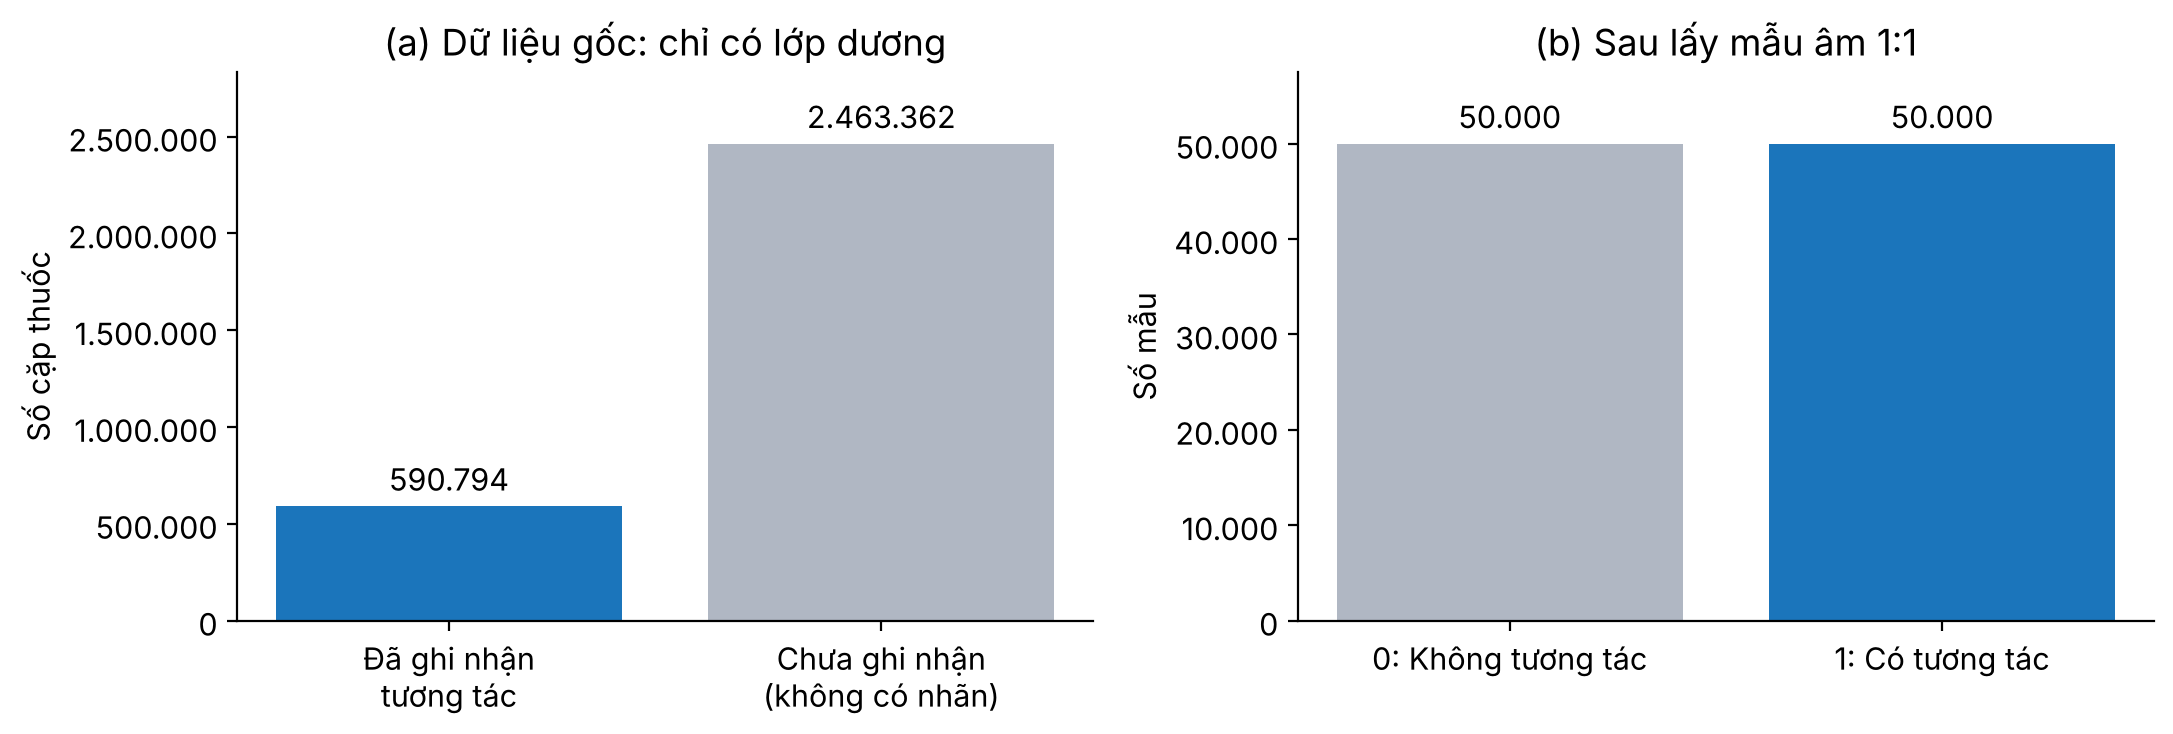
\includegraphics[width=\textwidth]{fig02_phan_bo_nhan.png}
  \caption{Phân bố nhãn: (a) dữ liệu gốc, (b) sau khi lấy mẫu âm}
  \label{fig:phanbonhan}
\end{figure}

\textit{Nhận xét:} Hình~\ref{fig:phanbonhan}a cho thấy DrugBank chỉ ghi nhận
\emph{lớp dương}: 590.794 cặp có tương tác (19,34\% trong 3.054.156 cặp có thể
ghép từ 2.472 thuốc), 80,66\% cặp còn lại không có nhãn -- không có cặp nào
được xác nhận ``không tương tác''. Do đó phải tạo mẫu âm (Mục~\ref{sec:chatluong}).
Sau khi lấy 50.000 cặp dương và 50.000 cặp âm (Hình~\ref{fig:phanbonhan}b), hai
lớp cân bằng tuyệt đối, nên không cần kỹ thuật cân bằng lớp ở bước huấn luyện.

\begin{figure}[H]
  \centering
  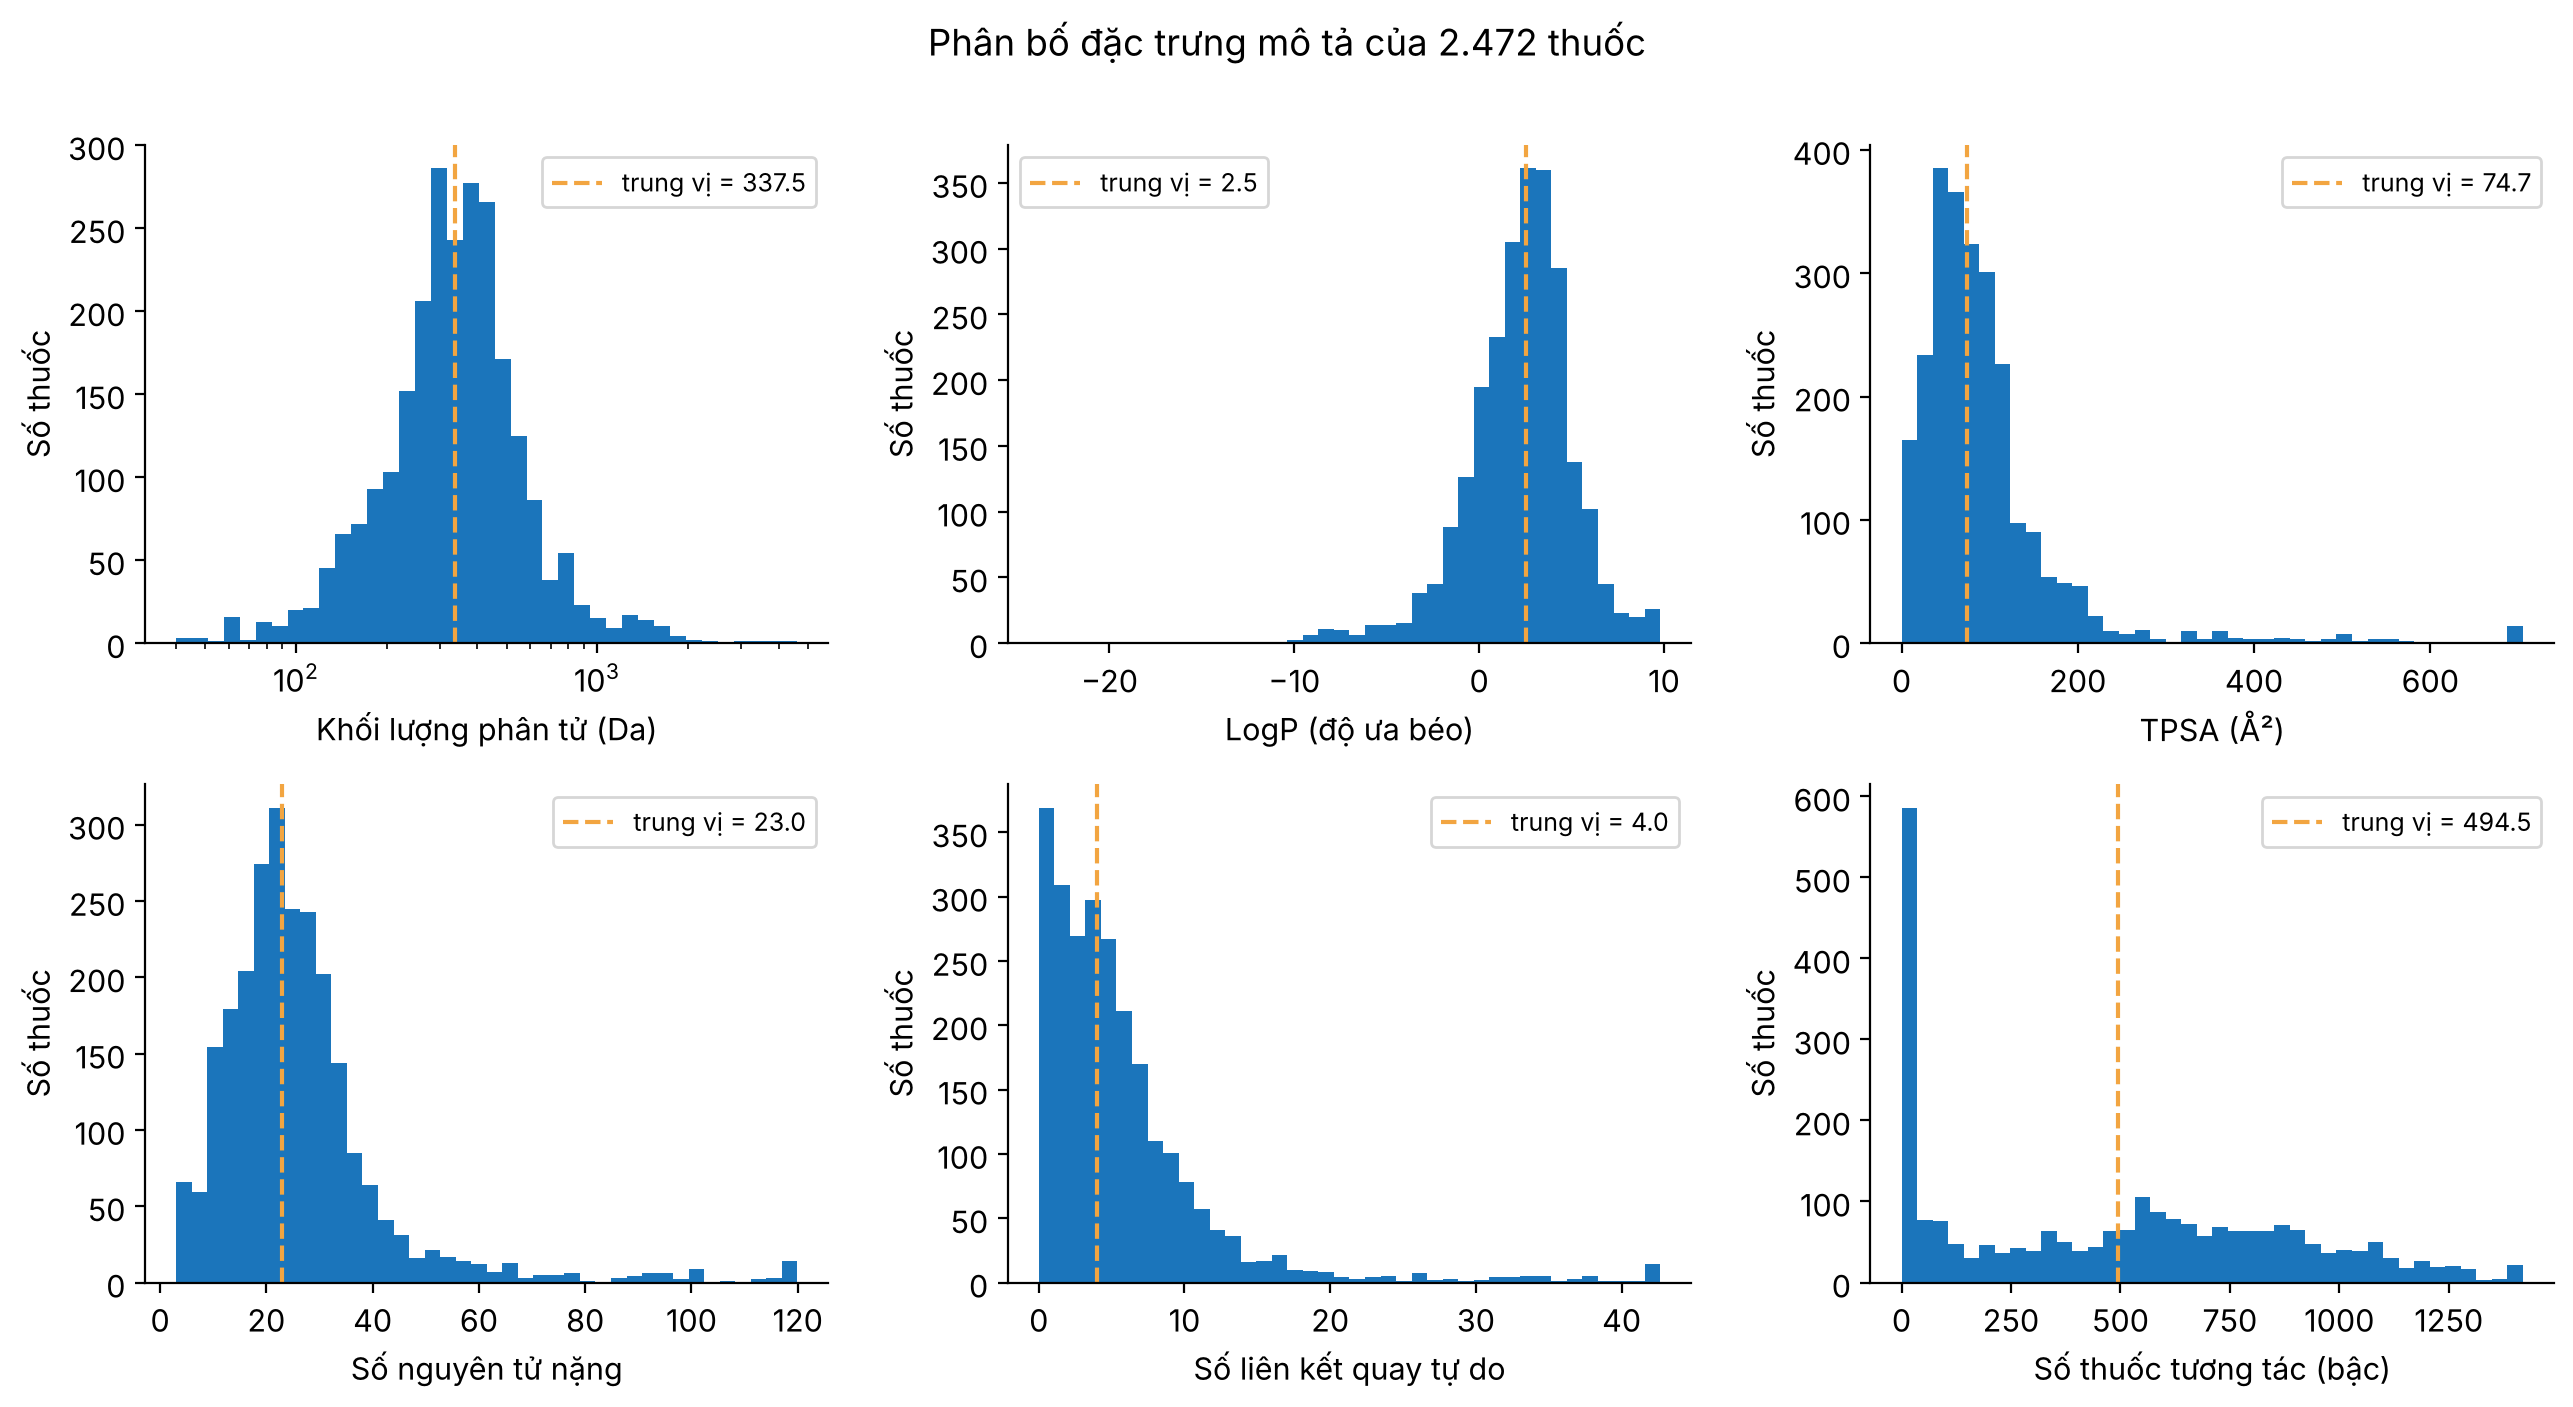
\includegraphics[width=\textwidth]{fig03_phan_bo_mo_ta.png}
  \caption{Phân bố các đặc trưng mô tả chính của thuốc}
  \label{fig:phanbomota}
\end{figure}

\textit{Nhận xét:} Theo Hình~\ref{fig:phanbomota}:
\begin{itemize}
  \item \textbf{Khối lượng phân tử} lệch phải mạnh (độ lệch 5,48): đa số thuốc
        nằm trong khoảng 248--446 Da (trung vị 337 Da, phù hợp quy tắc
        ``thuốc giống thuốc'' $<500$ Da), nhưng có đuôi dài gồm các peptide lớn
        như Imetelstat (4.610 Da), Semaglutide (4.114 Da).
  \item \textbf{LogP} tập trung quanh 2,5 (thuốc ưa béo vừa phải), có một số giá
        trị âm rất lớn ở các phân tử nhiều nhóm phân cực.
  \item \textbf{TPSA, số nguyên tử nặng, số liên kết quay} đều lệch phải và có
        đuôi dài cùng nhóm phân tử lớn; trung vị lần lượt 74,7 Å$^2$, 23 nguyên tử
        và 4 liên kết.
  \item \textbf{Bậc tương tác} phân bố hai đỉnh: 414 thuốc (16,7\%) có bậc 0
        (không tương tác với thuốc nào trong phạm vi), phần còn lại trải rộng
        tới 1.619. Đây là dấu hiệu quan trọng cho việc tạo mẫu âm (Mục~\ref{sec:chatluong}).
\end{itemize}

\begin{figure}[H]
  \centering
  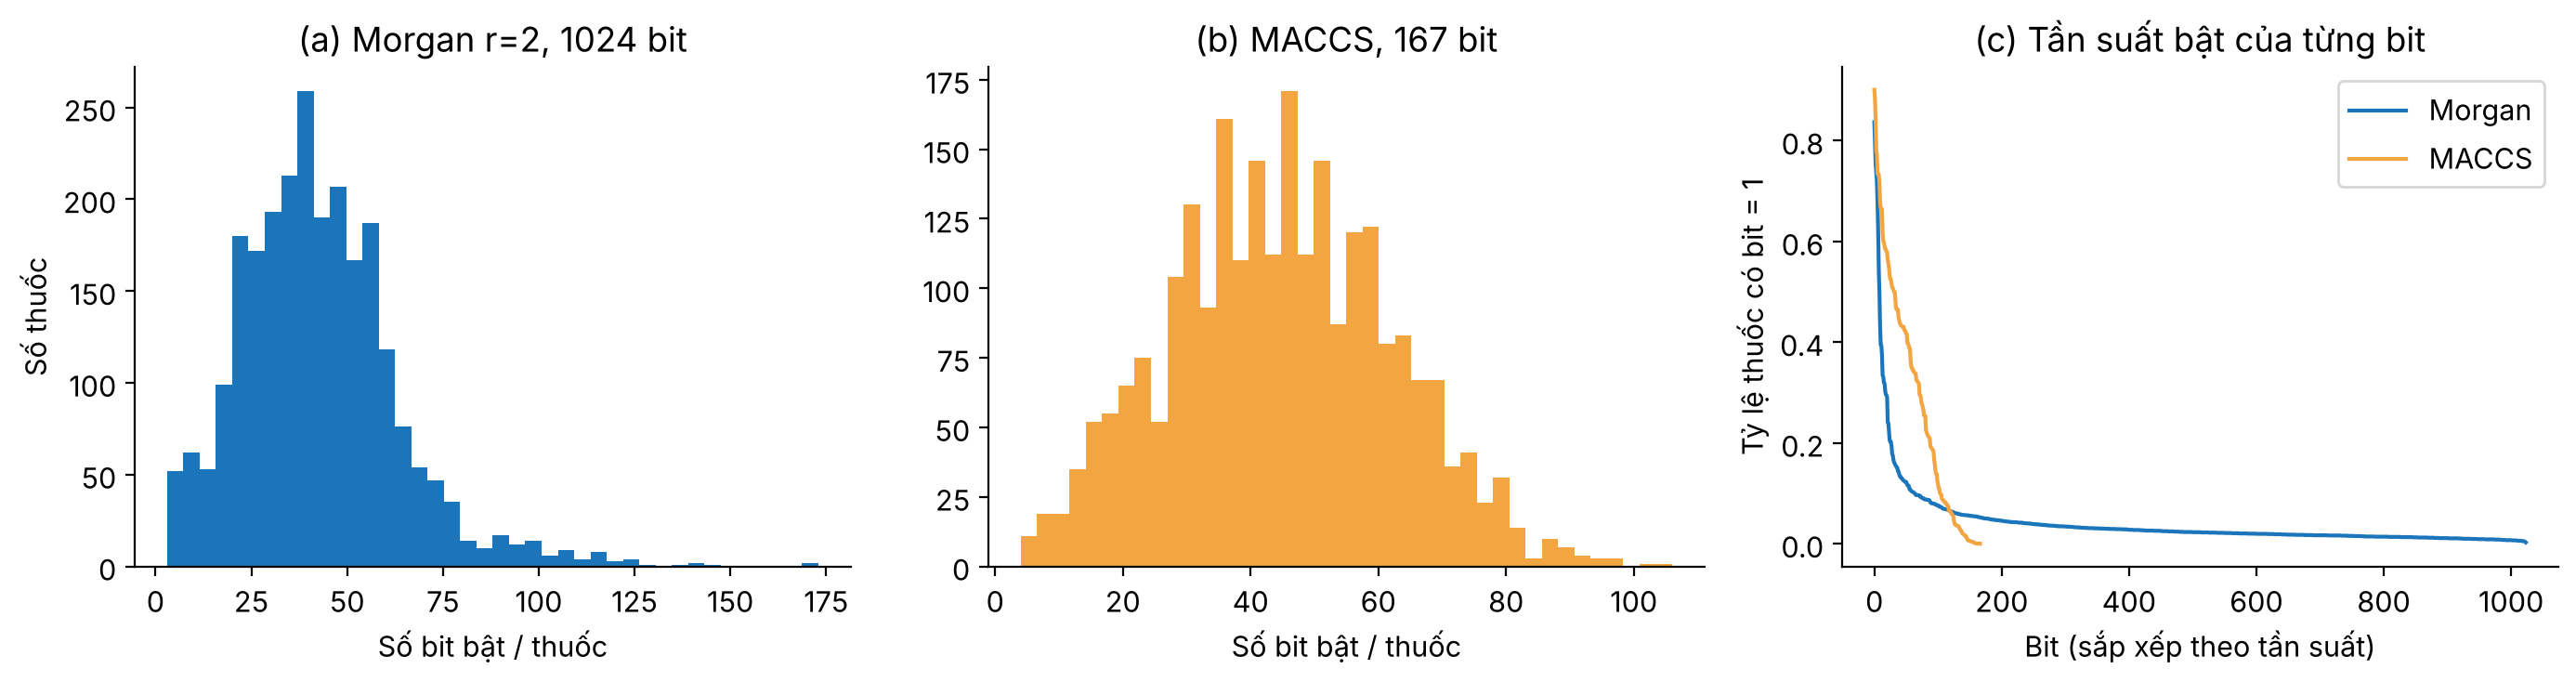
\includegraphics[width=\textwidth]{fig04_fingerprint.png}
  \caption{Đặc trưng vân tay phân tử: số bit bật mỗi thuốc và tần suất bật của từng bit}
  \label{fig:fingerprint}
\end{figure}

\textit{Nhận xét:} Hình~\ref{fig:fingerprint} cho thấy vân tay Morgan rất
\emph{thưa}: trung vị 40/1.024 bit bằng 1 mỗi thuốc, mật độ trung bình 4,15\%,
đa số bit chỉ bật ở dưới 5\% số thuốc. MACCS dày hơn (trung vị 44/167 bit, mật
độ 26,78\%), một số khóa bật ở trên 80\% thuốc (vd. có vòng), trong khi 6 khóa
không bao giờ bật. Đặc trưng thưa, nhị phân phù hợp với mô hình cây và mô hình
tuyến tính có điều chuẩn.

\subsection{Quan hệ giữa các đặc trưng}

\begin{figure}[H]
  \centering
  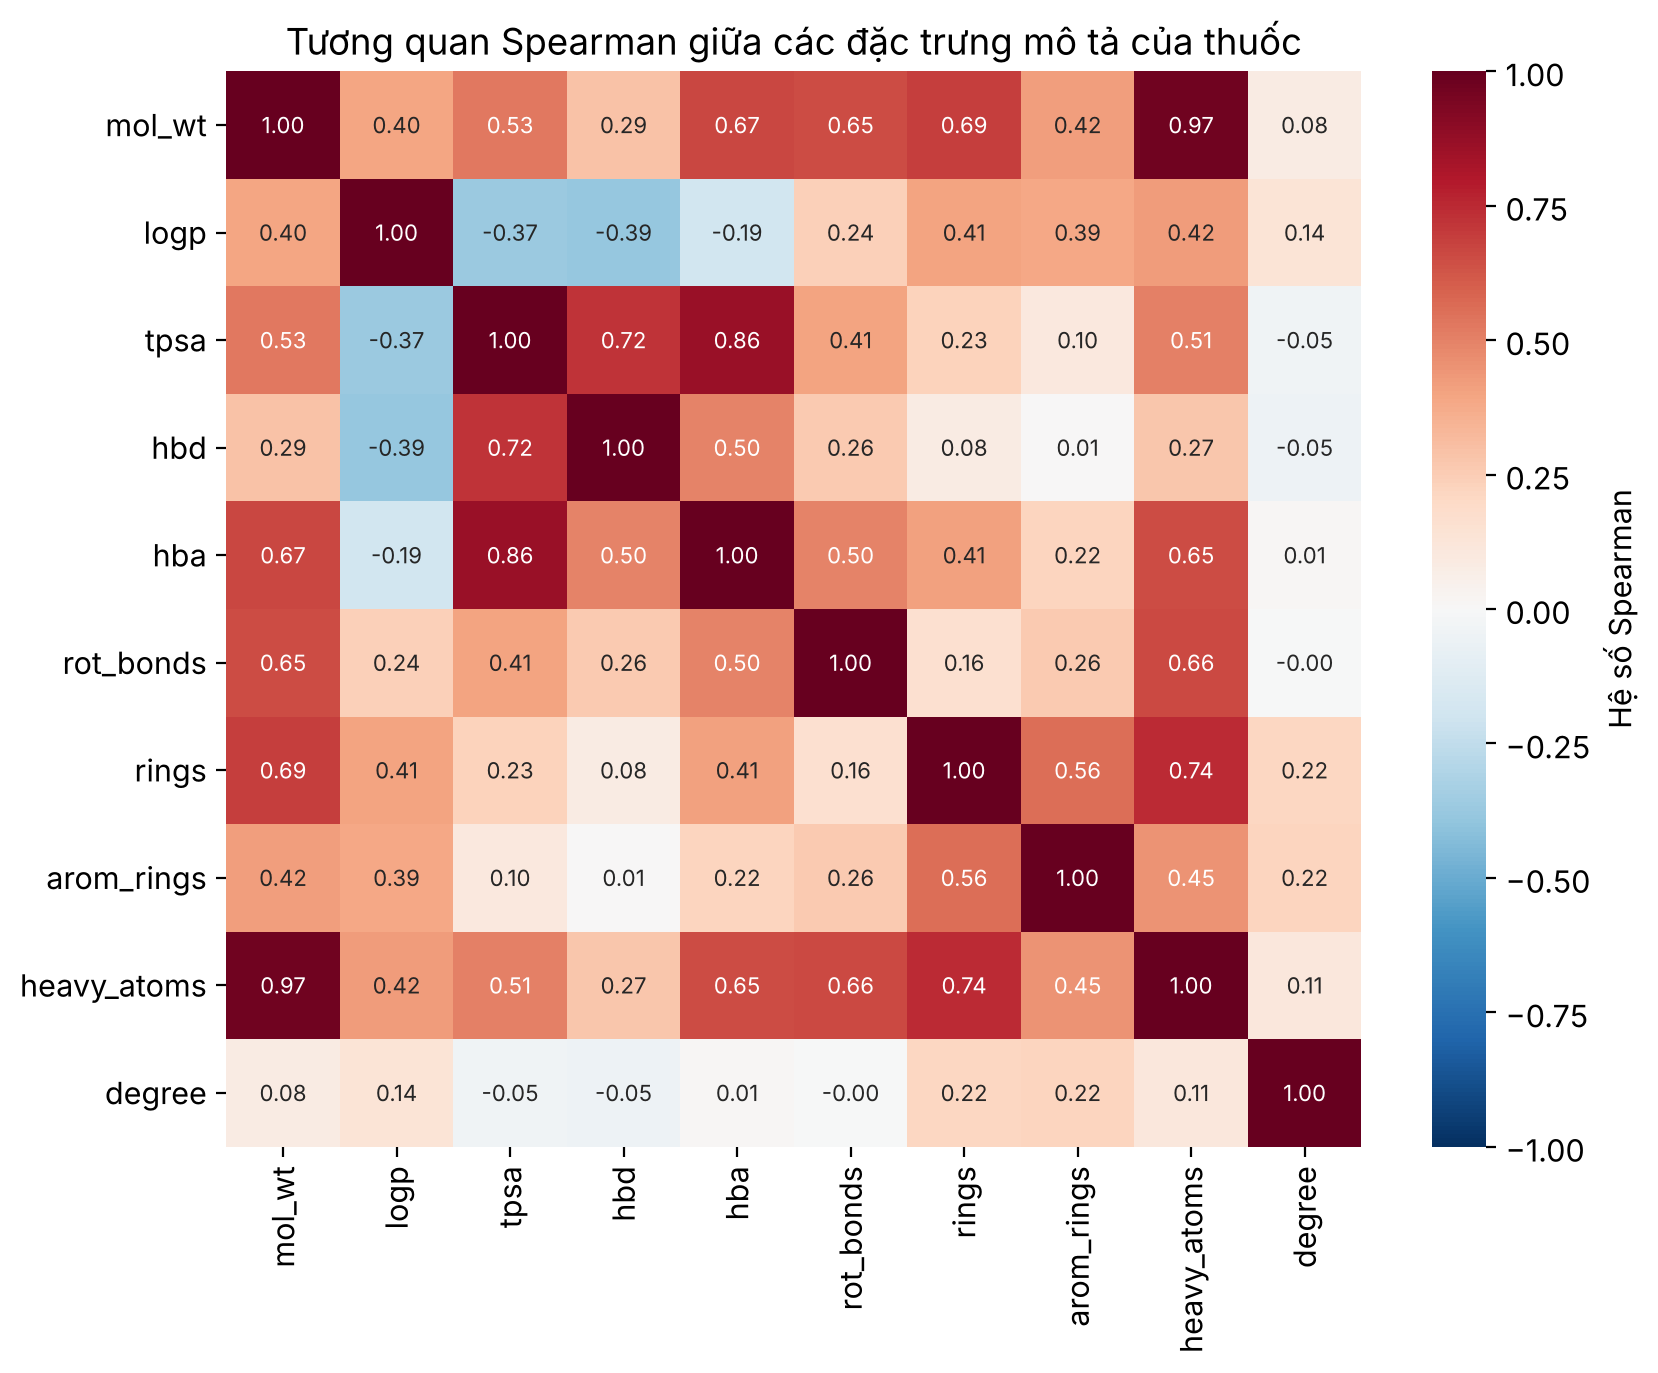
\includegraphics[width=0.78\textwidth]{fig05_tuong_quan.png}
  \caption{Ma trận tương quan Spearman giữa các đặc trưng mô tả của thuốc}
  \label{fig:tuongquan}
\end{figure}

\begin{figure}[H]
  \centering
  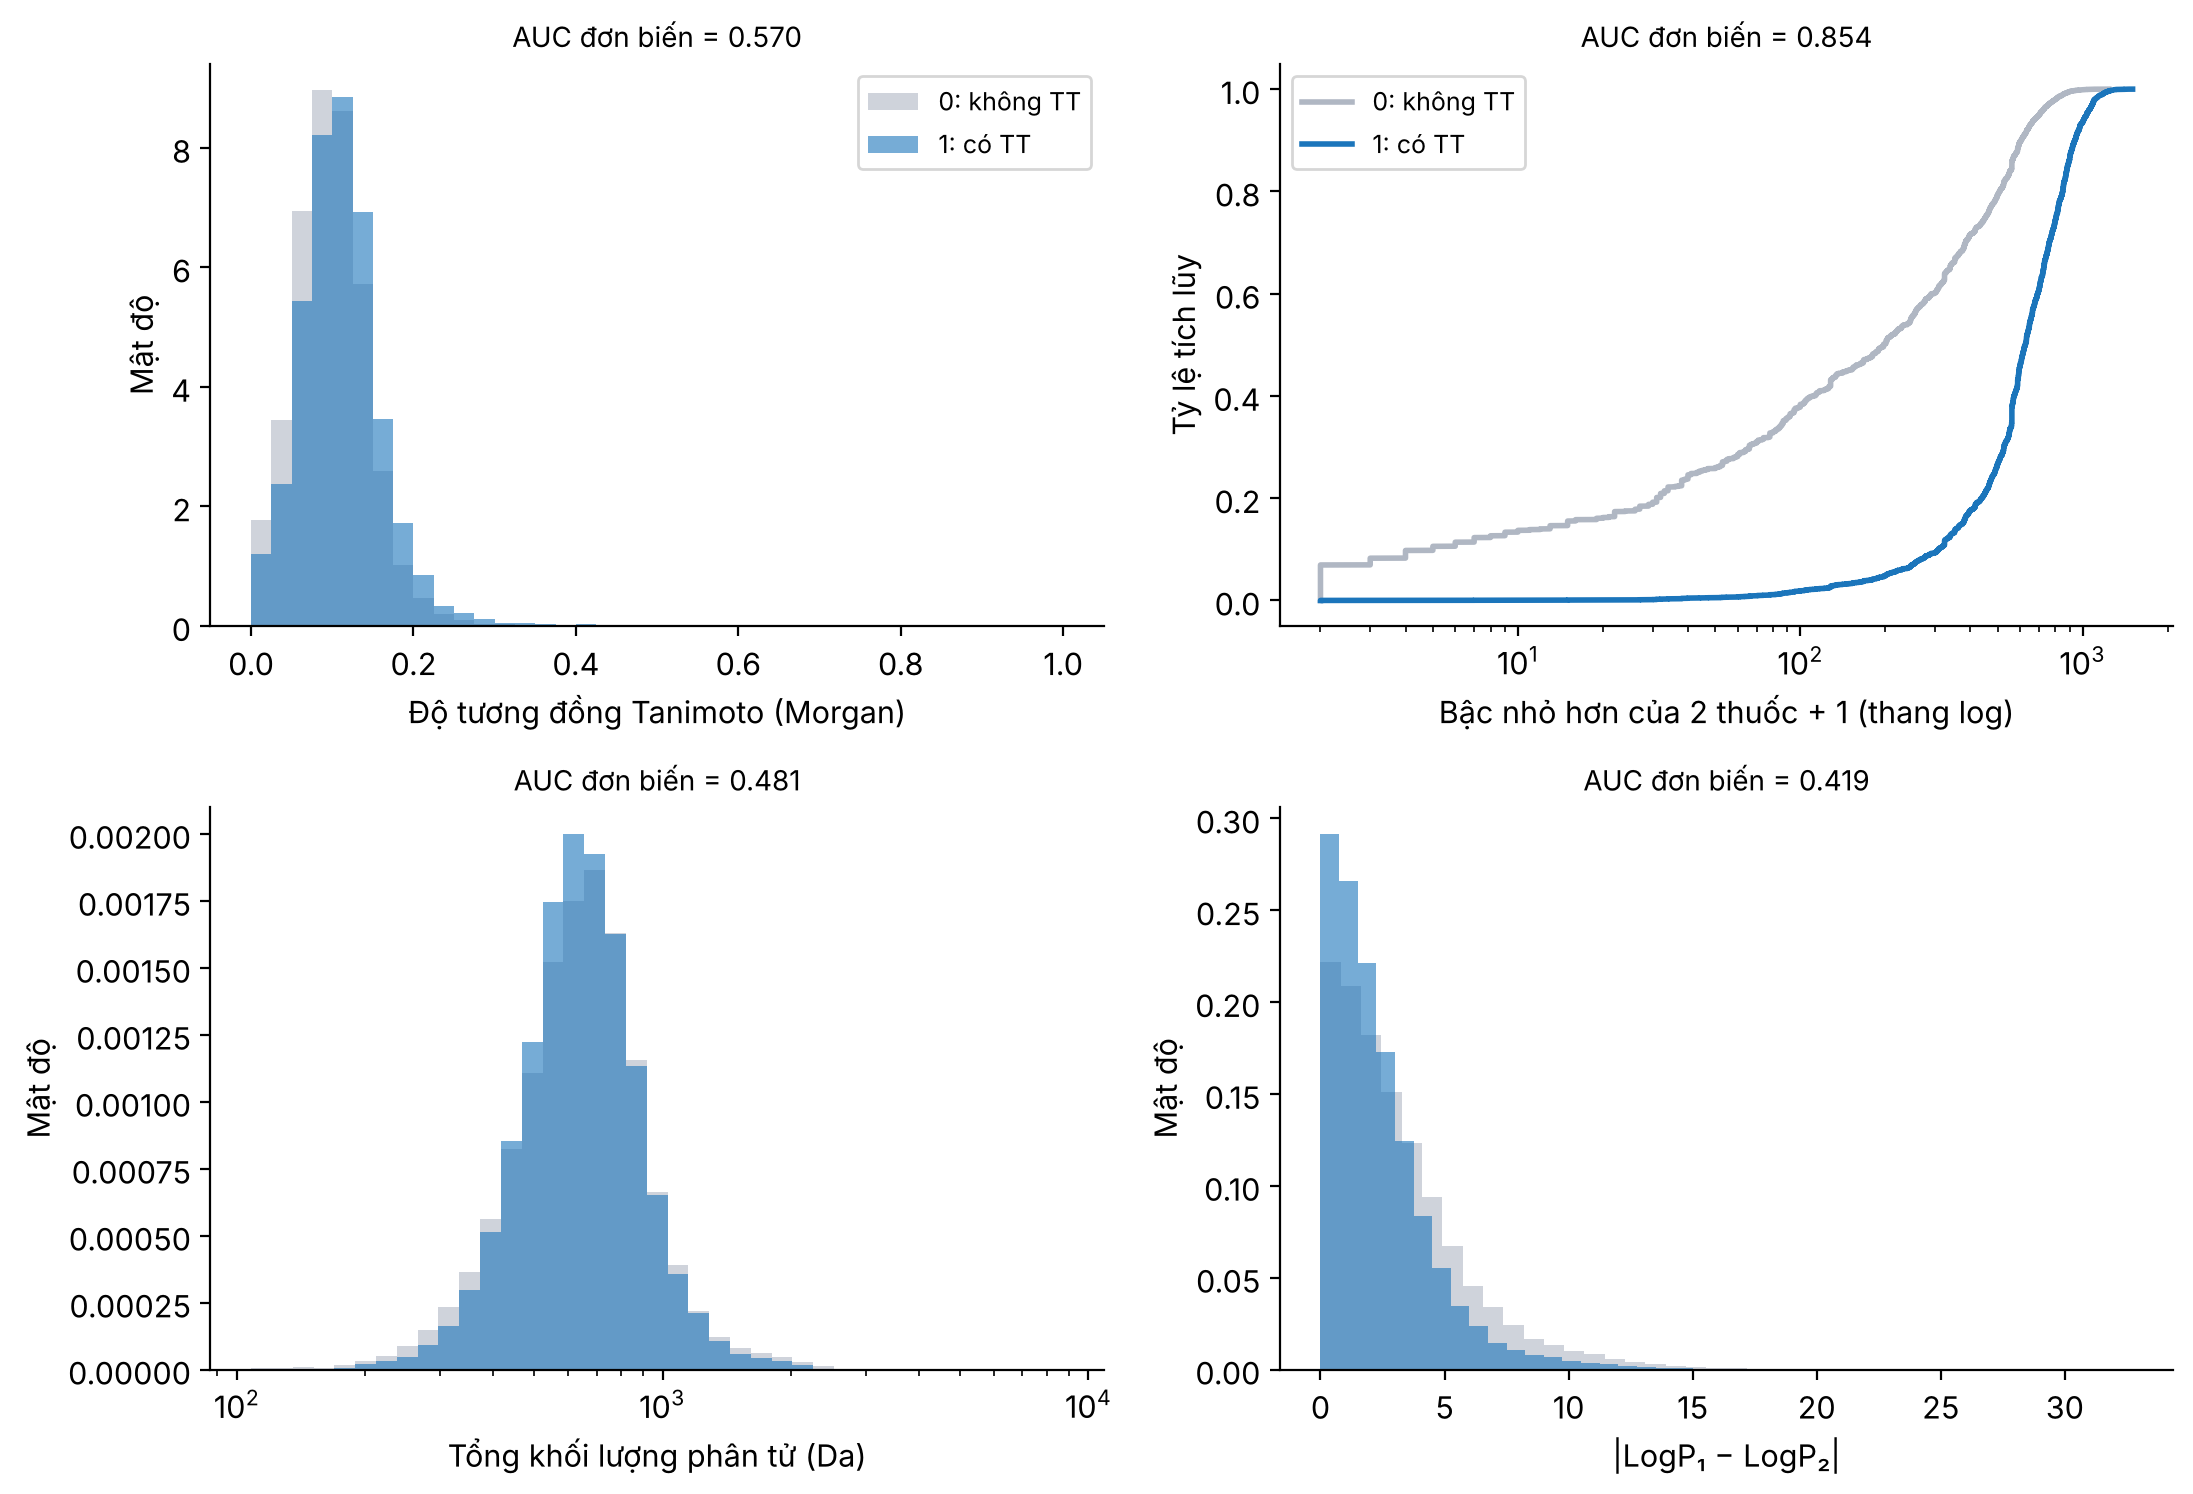
\includegraphics[width=0.92\textwidth]{fig06_dac_trung_cap_theo_nhan.png}
  \caption{Phân bố đặc trưng ở mức cặp thuốc theo nhãn (kèm AUC đơn biến)}
  \label{fig:capnhan}
\end{figure}

\begin{table}[H]
  \centering
  \caption{Đặc trưng ở mức cặp thuốc theo nhãn và AUC khi dùng riêng từng đặc trưng}
  \label{tab:donbien}
  \small
  \begin{tabular}{lccc}
    \toprule
    \textbf{Đặc trưng cặp} & \textbf{TB lớp 1} & \textbf{TB lớp 0} & \textbf{AUC đơn biến} \\
    \midrule
    Độ tương đồng Tanimoto (Morgan) & 0,111 & 0,099 & 0,570 \\
    Bậc nhỏ hơn của hai thuốc & 631,1 & 260,6 & 0,854 \\
    Tổng bậc hai thuốc & 1.613,0 & 965,6 & 0,858 \\
    Tổng khối lượng phân tử (Da) & 761,6 & 801,7 & 0,481 \\
    $|\text{LogP}_A-\text{LogP}_B|$ & 2,42 & 3,16 & 0,419 \\
    Tổng TPSA (Å$^2$) & 172,8 & 201,3 & 0,436 \\
    \bottomrule
  \end{tabular}
\end{table}

\begin{figure}[H]
  \centering
  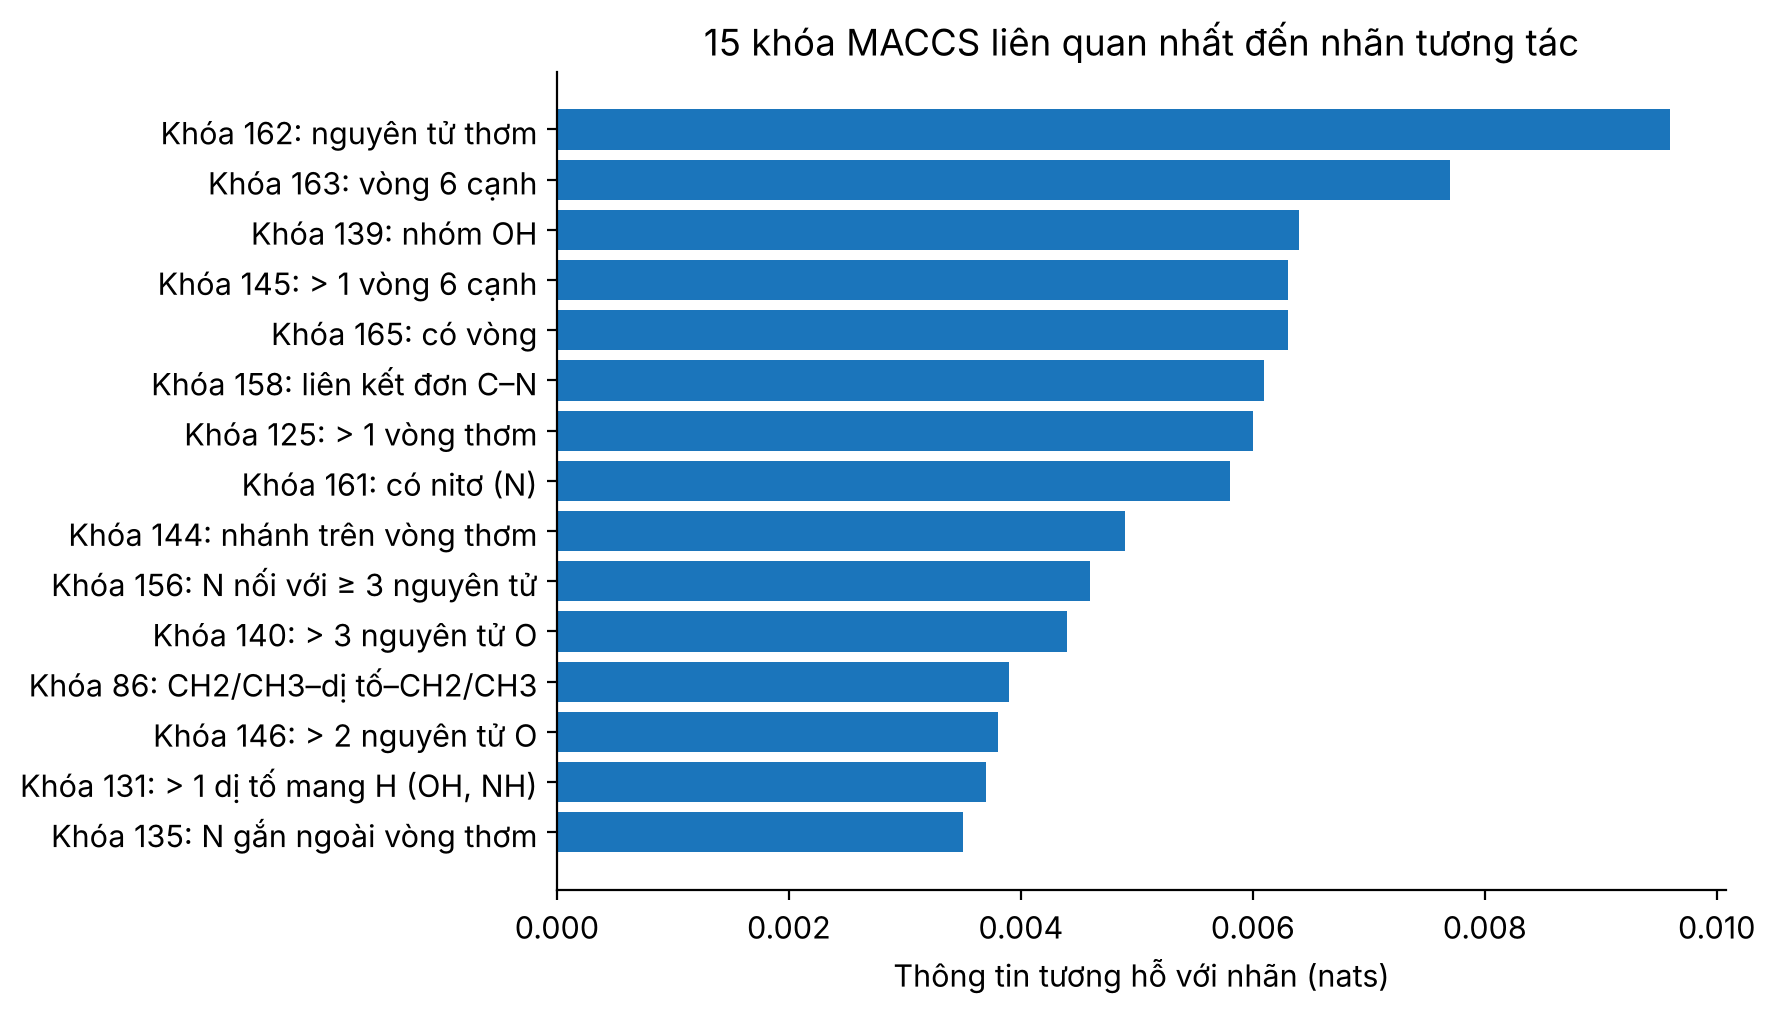
\includegraphics[width=0.85\textwidth]{fig07_maccs_mi.png}
  \caption{15 khóa MACCS có thông tin tương hỗ lớn nhất với nhãn}
  \label{fig:maccsmi}
\end{figure}

\textit{Nhận xét} (Hình~\ref{fig:tuongquan}--\ref{fig:maccsmi}, Bảng~\ref{tab:donbien}):
\begin{enumerate}
  \item \textbf{Đặc trưng mô tả dư thừa:} khối lượng phân tử và số nguyên tử nặng
        tương quan gần tuyệt đối ($\rho=0{,}97$), TPSA tương quan mạnh với số nhóm
        nhận liên kết hydro ($\rho=0{,}86$) và cho liên kết hydro ($\rho=0{,}72$).
        Tương tự, có 22 cặp khóa MACCS tương quan $|r|>0{,}9$. Thông tin cấu trúc
        bị lặp lại nhiều, nên mô hình tuyến tính cần điều chuẩn và có thể cân
        nhắc lựa chọn đặc trưng ở giai đoạn cải tiến.
  \item \textbf{Mỗi bit cấu trúc riêng lẻ chỉ liên quan yếu đến nhãn:} khóa MACCS
        mạnh nhất (khóa 162 -- có nguyên tử thơm) chỉ có MI = 0,0096 nats; các cặp
        tương tác có nhiều vòng thơm hơn (khóa 125 ``>1 vòng thơm'': 78,6\% so
        với 72,9\%) và ít nhóm OH, ít nguyên tử O hơn (khóa 139: 70,3\% so với
        79,4\%). Độ tương đồng Tanimoto giữa hai thuốc cũng chỉ đạt AUC 0,570.
        Vì vậy cần mô hình đa biến, phi tuyến (Random Forest, XGBoost) để kết hợp
        nhiều bit, thay vì dựa vào một vài đặc trưng.
  \item \textbf{Bậc tương tác của thuốc dự đoán nhãn rất mạnh} (AUC đơn biến 0,854
        với bậc nhỏ hơn): các thuốc ``phổ biến'' tham gia nhiều cặp dương, trong
        khi mẫu âm ngẫu nhiên hay chứa thuốc ít tương tác. Bậc được tính từ chính
        nhãn nên \emph{không được dùng làm đặc trưng} (rò rỉ nhãn); tuy nhiên mô
        hình vẫn có thể gián tiếp học ``độ phổ biến'' của thuốc qua vân tay. Đây là
        thiên lệch cần kiểm soát khi tạo mẫu âm và khi đánh giá theo nhóm thuốc.
  \item \textbf{Đặc trưng kích thước phân tử gần như không phân biệt nhãn} (tổng
        khối lượng phân tử AUC 0,481), nên ngoại lai về kích thước không phải là
        nguồn tín hiệu chính; giữ lại các phân tử lớn không làm lệch mô hình.
  \item \textbf{Bậc gần như độc lập với đặc trưng mô tả} ($|\rho|\leq0{,}22$): độ
        phổ biến của thuốc không giải thích được bằng kích thước hay độ phân cực,
        nghĩa là tín hiệu ``bậc'' và tín hiệu cấu trúc là hai nguồn khác nhau.
\end{enumerate}

\section{Phát hiện và xử lý vấn đề chất lượng dữ liệu}
\label{sec:chatluong}
Các vấn đề chất lượng dữ liệu được định lượng và xử lý như trong
Bảng~\ref{tab:chatluong}; so sánh trước -- sau xử lý ở Hình~\ref{fig:truocsau}.

{\small
\begin{xltabular}{\textwidth}{p{3.4cm} >{\centering\arraybackslash}p{2.6cm} X}
\caption{Thống kê các vấn đề chất lượng dữ liệu và cách xử lý}\label{tab:chatluong}\\
\toprule
\textbf{Vấn đề} & \textbf{Số lượng (tỷ lệ)} & \textbf{Cách xử lý và lý do} \\ \midrule
\endfirsthead
\multicolumn{3}{l}{\textit{Bảng \thetable\ (tiếp theo)}}\\ \toprule
\textbf{Vấn đề} & \textbf{Số lượng (tỷ lệ)} & \textbf{Cách xử lý và lý do} \\ \midrule
\endhead
\bottomrule
\endlastfoot
    Bản ghi tương tác trùng (A--B và B--A) & 1.427.655 / 2.855.848 (49,99\%) & Gộp thành cặp không thứ tự (A < B). Nếu giữ cả hai chiều, cùng một tương tác có thể rơi vào cả tập train và test, gây rò rỉ. \\
    Cặp tham chiếu thuốc không có trong bảng thuốc & 538 / 1.428.193 (0,04\%) & Loại bỏ vì không có thông tin cấu trúc. \\
    Thiếu SMILES & 5.117 / 17.430 (29,36\%); trong phạm vi: 157 / 2.802 (5,60\%) & Chủ yếu là thuốc sinh học (4.264). Giới hạn phạm vi vào thuốc phân tử nhỏ đã phê duyệt, loại 157 thuốc thiếu SMILES: không thể điền khuyết cấu trúc hóa học. \\
    SMILES không hợp lệ & 2 / 2.802 (0,07\%) & Loại bỏ (RDKit không đọc được). \\
    SMILES nhiều thành phần (muối, nước kết tinh) & 246 / 2.802 (8,78\%) & Giữ thành phần lớn nhất (\texttt{LargestFragmentChooser}): ion đối như Na$^+$, Cl$^-$ không quyết định hoạt tính nhưng làm vân tay khác nhau giữa các dạng muối. \\
    Thành phần chính quá nhỏ ($\leq2$ nguyên tử nặng) & 84 / 2.802 (3,00\%) & Loại bỏ (ion, chất vô cơ như K, Fe, NaCl): vân tay gần như toàn 0, không mang thông tin cấu trúc. \\
    Trùng cấu trúc (khác mã, cùng phân tử) & 87 mã thừa (3,10\%), 129 mã thuộc 42 cấu trúc & Gộp về một mã đại diện (mã có nhiều tương tác nhất), ánh xạ cặp tương tác sang mã đại diện. Nếu không, các mẫu có đặc trưng giống hệt nhau xuất hiện ở cả train và test. \\
    Ngoại lai kích thước phân tử (IQR) & \texttt{mol\_wt}: 154 (6,2\%); \texttt{tpsa}: 135 (5,5\%) & Giữ lại: đây là thuốc thật (peptide, kháng sinh lớn); vân tay là đặc trưng nhị phân nên không bị ảnh hưởng bởi độ lớn giá trị; kích thước gần như không liên quan đến nhãn (Bảng~\ref{tab:donbien}). \\
    Mất cân bằng lớp & 100\% dương; 0 cặp âm được ghi nhận & Lấy mẫu âm 1:1 từ các cặp chưa ghi nhận tương tác (loại mọi cặp có trong DrugBank). \\
    Thiên lệch khi lấy mẫu âm & 414 thuốc bậc 0; 37,9\% mẫu âm chứa thuốc bậc 0 & Chỉ ghép mẫu âm trong 2.058 thuốc có $\geq1$ tương tác (như Ran \textit{et al.}): tỷ lệ còn 0\%, AUC của ``bậc'' giảm từ 0,909 xuống 0,854 (Bảng~\ref{tab:mauam}). \\
    Nguy cơ rò rỉ khi chia theo cặp & 100\% thuốc của tập kiểm tra có mặt trong tập huấn luyện & Bổ sung đánh giá chia theo nhóm thuốc (Mục~\ref{sec:chuanbi}); không dùng mã thuốc, bậc làm đặc trưng. \\
\end{xltabular}
}

\begin{figure}[H]
  \centering
  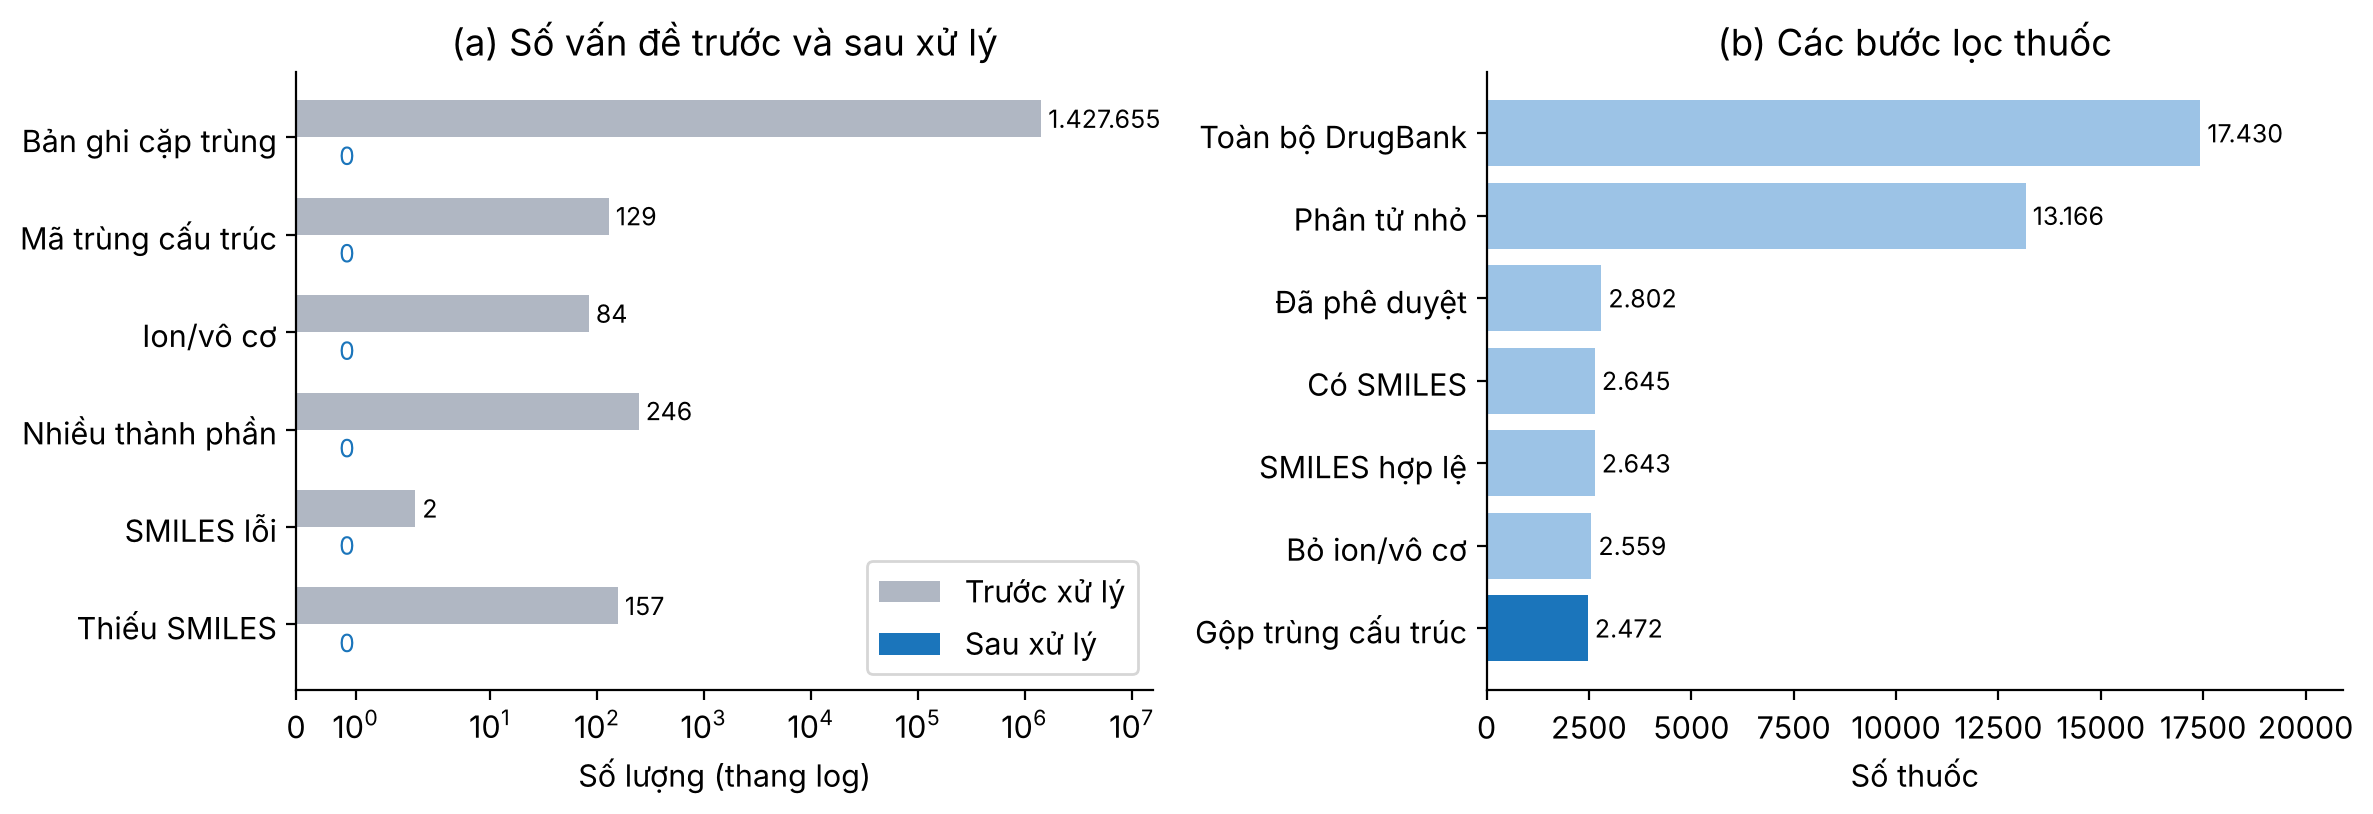
\includegraphics[width=\textwidth]{fig01_truoc_sau_lam_sach.png}
  \caption{So sánh trước -- sau xử lý: (a) số vấn đề, (b) số thuốc qua từng bước lọc}
  \label{fig:truocsau}
\end{figure}

\textit{Nhận xét:} Hình~\ref{fig:truocsau}a cho thấy toàn bộ các vấn đề đã phát
hiện đều được đưa về 0 sau xử lý. Hình~\ref{fig:truocsau}b thể hiện số thuốc
giảm từ 17.430 xuống 2.472 qua các bước lọc; bước giảm lớn nhất là giới hạn vào
thuốc đã phê duyệt (13.166 $\rightarrow$ 2.802). Việc ánh xạ mã trùng cấu trúc
làm giảm thêm 11.469 cặp tương tác trùng lặp, còn 590.794 cặp dương.

\begin{table}[H]
  \centering
  \caption{So sánh hai phương án lấy mẫu âm (cùng 50.000 cặp dương)}
  \label{tab:mauam}
  \small
  \begin{tabularx}{\textwidth}{X >{\centering\arraybackslash}p{2.4cm} >{\centering\arraybackslash}p{2.8cm} >{\centering\arraybackslash}p{2.8cm}}
    \toprule
    \textbf{Phương án} & \textbf{Số thuốc dùng để ghép} & \textbf{\% mẫu âm chứa thuốc bậc 0} & \textbf{AUC đơn biến của ``bậc nhỏ hơn''} \\
    \midrule
    1: Ghép ngẫu nhiên trong toàn bộ 2.472 thuốc & 2.472 & 37,9\% & 0,909 \\
    2 (chọn): Chỉ ghép trong thuốc có $\geq 1$ tương tác & 2.058 & 0,0\% & 0,854 \\
    \bottomrule
  \end{tabularx}
\end{table}

\textit{Nhận xét:} Với phương án 1, gần 38\% mẫu âm chứa một thuốc chưa từng
tương tác, mô hình có thể đạt điểm cao chỉ nhờ nhận ra ``thuốc lạ'' thay vì học
quan hệ cấu trúc. Phương án 2 loại bỏ hoàn toàn trường hợp này và giảm sức mạnh
dự đoán của ``bậc'' (AUC 0,909 $\rightarrow$ 0,854). Thiên lệch không mất hẳn
do thuốc phổ biến vẫn xuất hiện nhiều hơn ở lớp dương; nhóm sẽ đánh giá thêm
phương án lấy mẫu âm cân bằng theo bậc ở giai đoạn cải tiến (Bài kiểm tra 3).

\section{Chuẩn bị dữ liệu cho mô hình}
\label{sec:chuanbi}
\begin{itemize}
  \item \textbf{Mã hóa:} không có biến phân loại nào đưa vào mô hình; cấu trúc
        hóa học (SMILES) được mã hóa thành vân tay nhị phân Morgan (bán kính 2,
        1.024 bit) và MACCS (167 bit) bằng RDKit; vectơ cặp ghép nối hai thuốc
        theo thứ tự mã (2.382 chiều, kiểu \texttt{uint8}).
  \item \textbf{Chia tập:} hold-out phân tầng theo nhãn 80/20 với
        \texttt{random\_state = 42} (Bảng~\ref{tab:kichthuoc}); tập kiểm tra giữ
        nguyên đến đánh giá cuối. Ngoài ra, chia theo nhóm thuốc: chọn ngẫu nhiên
        20\% thuốc làm ``thuốc mới'', cặp có 1 hoặc 2 thuốc mới tạo thành tập
        S1, S2.
  \item \textbf{Lọc đặc trưng và chuẩn hóa:} \texttt{VarianceThreshold} và
        \texttt{StandardScaler} chỉ được \texttt{fit} trên tập huấn luyện rồi áp
        dụng cho tập kiểm tra: 16/2.382 bit luôn bằng 0 trên tập huấn luyện bị
        loại; sau chuẩn hóa, tập huấn luyện có trung bình 0, độ lệch chuẩn 1, tập
        kiểm tra có trung bình $\approx 0$, độ lệch chuẩn 1,001. Chuẩn hóa chỉ
        cần cho LR, SVM; khi huấn luyện, các bước này nằm trong \texttt{Pipeline}
        nên được fit lại trên từng fold huấn luyện.
\end{itemize}

\begin{table}[H]
  \centering
  \caption{Kích thước các tập dữ liệu sau khi chia}
  \label{tab:kichthuoc}
  \small
  \begin{tabular}{lccc}
    \toprule
    \textbf{Tập dữ liệu} & \textbf{Số mẫu} & \textbf{Số đặc trưng} & \textbf{Tỷ lệ lớp dương} \\
    \midrule
    Huấn luyện (hold-out) & 80.000 & 2.382 & 0,500 \\
    Kiểm tra (hold-out)   & 20.000 & 2.382 & 0,500 \\
    \midrule
    Theo thuốc: huấn luyện (2 thuốc đã biết) & 63.756 & 2.382 & 0,495 \\
    Theo thuốc: S1 (1 thuốc mới) & 32.208 & 2.382 & 0,508 \\
    Theo thuốc: S2 (2 thuốc mới) & 4.036 & 2.382 & 0,513 \\
    \bottomrule
  \end{tabular}
\end{table}

\begin{figure}[H]
  \centering
  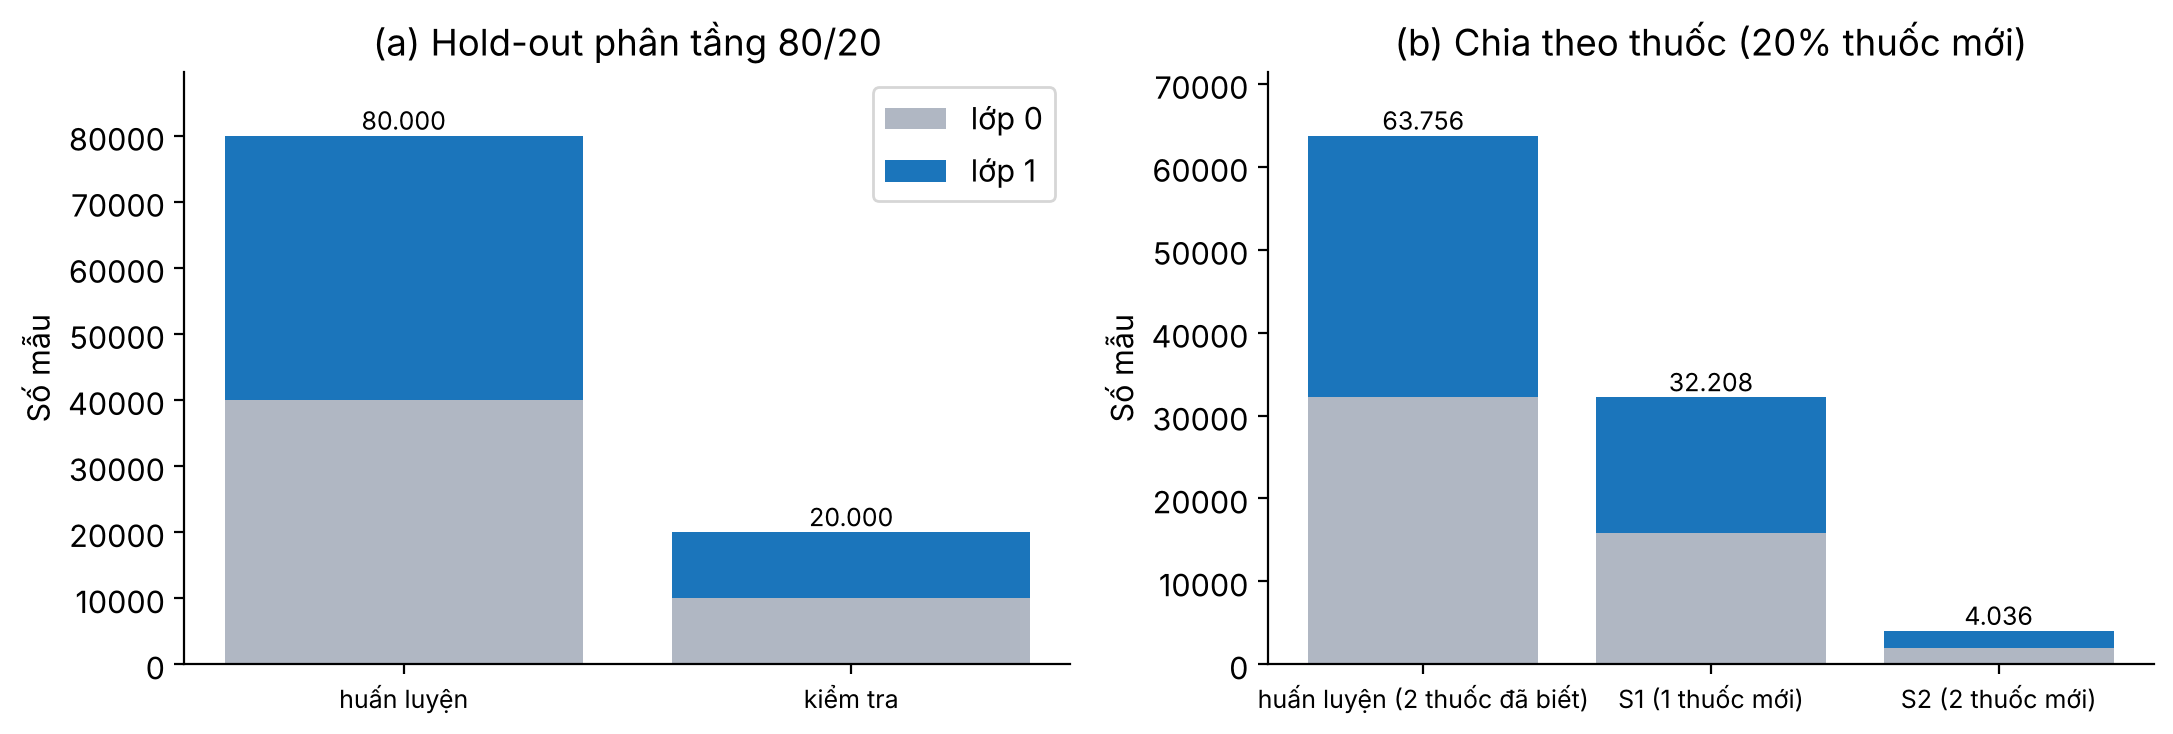
\includegraphics[width=\textwidth]{fig08_chia_tap.png}
  \caption{Kích thước và tỷ lệ lớp của các tập dữ liệu}
  \label{fig:chiatap}
\end{figure}

\textit{Nhận xét:} Hình~\ref{fig:chiatap}a cho thấy hai tập hold-out giữ đúng
tỷ lệ lớp 50/50 nhờ phân tầng. Khi chia theo cặp, toàn bộ thuốc của tập kiểm
tra đều đã xuất hiện trong tập huấn luyện, nên kết quả trên tập này phản ánh
khả năng dự đoán cho \emph{thuốc đã biết}. Các tập S1, S2 (Hình~\ref{fig:chiatap}b)
vẫn gần cân bằng và đủ lớn (4.036 cặp ở S2) để đo khả năng tổng quát hóa cho
thuốc mới.

\section{Môi trường thực nghiệm}
Notebook chạy trên CPU (2 nhân Intel Xeon 2,1~GHz), thời gian chạy toàn bộ khoảng
1 phút. Phần mềm: Python 3.13; NumPy 2.5; Pandas 3.0; Scikit-learn 1.9;
RDKit 2026.09; Matplotlib 3.11; Seaborn 0.13; XGBoost 3.4 (dùng từ Bài kiểm tra 2).
Mọi bước ngẫu nhiên dùng \texttt{random\_state = 42}. Cách chạy lại được trình bày ở
Phụ lục~\ref{pl:huongdan}.

\section{Kết quả huấn luyện và đánh giá}
\textit{Nội dung sẽ được trình bày ở Bài kiểm tra 2 (tuần 6): kết quả kiểm định
chéo 5-fold (trung bình $\pm$ độ lệch chuẩn) của mô hình cơ sở và các mô hình
LR, RF, SVM, XGBoost; ma trận nhầm lẫn, đường ROC.}

\section{Phân tích kết quả dự đoán}
\textit{Nội dung sẽ được trình bày ở Bài kiểm tra 2: phân tích lỗi theo bậc thuốc,
độ tương đồng, kích thước phân tử; so sánh train -- validation.}

\section{Tối ưu hóa và cải tiến mô hình}
\textit{Nội dung sẽ được trình bày ở Bài kiểm tra 3 (tuần 8): phân tích hạn chế,
cải tiến đặc trưng (Morgan dạng đếm, cách biểu diễn cặp, lấy mẫu âm cân bằng
theo bậc), thử nghiệm phương pháp tổ hợp, tối ưu siêu tham số bằng kiểm định chéo.}

\section{So sánh trước và sau cải tiến}
\textit{Nội dung sẽ được trình bày ở Bài kiểm tra 3.}

\section{Khả năng tổng quát hóa và lựa chọn mô hình cuối}
\textit{Nội dung sẽ được trình bày ở Bài kiểm tra 3: kết quả trên tập kiểm tra giữ
lại và các tập S1, S2.}

\section{Kết luận chương 3}
Ở giai đoạn 1, nhóm đã trích xuất dữ liệu DrugBank 5.1, phát hiện và định lượng
11 nhóm vấn đề chất lượng dữ liệu, xử lý từng vấn đề kèm lý do, thu được 2.472
thuốc và 590.794 cặp tương tác. Bộ dữ liệu mô hình gồm 100.000 cặp cân bằng,
2.382 đặc trưng nhị phân, chia hold-out phân tầng 80/20 và chia theo nhóm thuốc.
Khảo sát cho thấy tín hiệu cấu trúc phân tán trên nhiều bit (mỗi bit đơn lẻ liên
quan yếu đến nhãn) và tồn tại thiên lệch ``độ phổ biến của thuốc'' cần kiểm soát.

% =====================================================================
%  KẾT LUẬN
% =====================================================================
\unnumberedchapter{KẾT LUẬN VÀ HƯỚNG PHÁT TRIỂN}

\section*{1. Kết quả đạt được (giai đoạn 1)}
Nhóm đã phát biểu bài toán phân loại nhị phân trên cặp thuốc, xác định mục tiêu
và chỉ số đánh giá (ROC-AUC $\geq 0{,}85$, F1 $\geq 0{,}80$), xây dựng bộ dữ liệu
100.000 cặp thuốc sạch từ DrugBank 5.1 kèm từ điển dữ liệu, thống kê mô tả, phân
tích quan hệ đặc trưng -- nhãn và chuẩn bị dữ liệu đúng quy trình không rò rỉ.

\section*{2. Hạn chế}
Mẫu âm là các cặp \emph{chưa ghi nhận} tương tác, có thể lẫn tương tác có thật
chưa được phát hiện; thiên lệch theo bậc của thuốc chưa được loại bỏ hoàn toàn;
đề tài chỉ dùng thông tin cấu trúc hóa học.

\section*{3. Hướng phát triển}
Ở các giai đoạn tiếp theo: huấn luyện và so sánh bốn thuật toán với mô hình cơ
sở (Bài kiểm tra 2); thử lấy mẫu âm cân bằng theo bậc, các cách biểu diễn cặp
khác, phương pháp tổ hợp và tối ưu siêu tham số (Bài kiểm tra 3). Về lâu dài có
thể bổ sung đặc trưng protein đích, enzyme của thuốc.

% =====================================================================
%  TÀI LIỆU THAM KHẢO
% =====================================================================
\begin{thebibliography}{99}
\setlength{\itemsep}{2pt}

\bibitem{breiman2001}
L.~Breiman (2001), ``Random forests'', \textit{Machine Learning}, vol.~45,
no.~1, pp.~5--32.

\bibitem{chen2016}
T.~Chen, C.~Guestrin (2016), ``XGBoost: A scalable tree boosting system'',
in \textit{Proceedings of the 22nd ACM SIGKDD International Conference on
Knowledge Discovery and Data Mining}, pp.~785--794.

\bibitem{cheng2014}
F.~Cheng, Z.~Zhao (2014), ``Machine learning-based prediction of drug--drug
interactions by integrating drug phenotypic, therapeutic, chemical, and genomic
properties'', \textit{Journal of the American Medical Informatics Association},
vol.~21, no.~e2, pp.~e278--e286.

\bibitem{cortes1995}
C.~Cortes, V.~Vapnik (1995), ``Support-vector networks'', \textit{Machine
Learning}, vol.~20, no.~3, pp.~273--297.

\bibitem{durant2002}
J.~L.~Durant, B.~A.~Leland, D.~R.~Henry, J.~G.~Nourse (2002), ``Reoptimization
of MDL keys for use in drug discovery'', \textit{Journal of Chemical Information
and Computer Sciences}, vol.~42, no.~6, pp.~1273--1280.

\bibitem{rdkit}
G.~Landrum, ``RDKit: Open-source cheminformatics'', \url{https://www.rdkit.org}.

\bibitem{pedregosa2011}
F.~Pedregosa \textit{et al.} (2011), ``Scikit-learn: Machine learning in
Python'', \textit{Journal of Machine Learning Research}, vol.~12,
pp.~2825--2830.

\bibitem{ran2022}
B.~Ran, L.~Chen, M.~Li, Y.~Han, Q.~Dai (2022), ``Drug-drug interactions
prediction using fingerprint only'', \textit{Computational and Mathematical
Methods in Medicine}, vol.~2022, Article ID 7818480.

\bibitem{rogers2010}
D.~Rogers, M.~Hahn (2010), ``Extended-connectivity fingerprints'',
\textit{Journal of Chemical Information and Modeling}, vol.~50, no.~5,
pp.~742--754.

\bibitem{ryu2018}
J.~Y.~Ryu, H.~U.~Kim, S.~Y.~Lee (2018), ``Deep learning improves prediction of
drug--drug and drug--food interactions'', \textit{Proceedings of the National
Academy of Sciences}, vol.~115, no.~18, pp.~E4304--E4311.

\bibitem{vilar2012}
S.~Vilar, R.~Harpaz, E.~Uriarte, L.~Santana, R.~Rabadan, C.~Friedman (2012),
``Drug--drug interaction through molecular structure similarity analysis'',
\textit{Journal of the American Medical Informatics Association}, vol.~19,
no.~6, pp.~1066--1074.

\bibitem{wishart2018}
D.~S.~Wishart \textit{et al.} (2018), ``DrugBank 5.0: a major update to the
DrugBank database for 2018'', \textit{Nucleic Acids Research}, vol.~46,
no.~D1, pp.~D1074--D1082.

\end{thebibliography}

% =====================================================================
%  PHỤ LỤC
% =====================================================================
\appendix
\renewcommand{\bmchapname}{Phụ lục}
\addtocontents{toc}{\protect\renewcommand{\protect\tocchapname}{\appendixname}}

\chapter{Hướng dẫn cài đặt và chạy chương trình}
\label{pl:huongdan}

\section{Yêu cầu môi trường}
\begin{itemize}
  \item Python $\geq$ 3.10; các thư viện liệt kê trong \texttt{requirements.txt}
        (NumPy, Pandas, Scikit-learn, RDKit, Matplotlib, Seaborn, lxml).
  \item Mã nguồn và dữ liệu: nộp kèm trong thư mục bài nộp (\texttt{Nhom 05.zip}).
  \item Dữ liệu đã trích xuất có sẵn trong thư mục \texttt{data/raw/}; file gốc
        \texttt{full database.xml} cần tải từ DrugBank (yêu cầu tài khoản học thuật).
\end{itemize}

\section{Các bước thực hiện}
Cấu trúc thư mục nộp bài:
\begin{lstlisting}[language=bash,numbers=none]
Nhom 05/
  BaoCao_Nhom_05.pdf            # bao cao
  LaTeX/                        # ma nguon LaTeX + hinh (images/)
  data/raw/                     # drugs.csv, ddi_pairs.csv.gz, meta.txt
  data/processed/               # du lieu sau xu ly (notebook tao ra)
  notebooks/01_EDA_TienXuLy.ipynb
  src/extract_drugbank.py       # trich xuat tu DrugBank XML
  requirements.txt, README.md, PhanCong_NhatKy.md
\end{lstlisting}

Bước 1: cài đặt thư viện:
\begin{lstlisting}[language=bash,numbers=none]
pip install -r requirements.txt
\end{lstlisting}
Bước 2 (tùy chọn, chỉ khi muốn trích xuất lại từ file gốc):
\begin{lstlisting}[language=bash,numbers=none]
python src/extract_drugbank.py "duong/dan/full database.xml" data/raw
\end{lstlisting}
Bước 3: mở \texttt{notebooks/01\_EDA\_TienXuLy.ipynb} bằng Jupyter/VS Code và
chọn \textit{Run All}. Notebook đọc \texttt{data/raw/}, ghi kết quả vào
\texttt{data/processed/} và hình vào \texttt{LaTeX/images/}.

\chapter{Nhật ký đóng góp của các thành viên}
\label{pl:nhatky}

\begin{table}[H]
  \centering
  \caption{Nhật ký công việc giai đoạn 1}
  \label{tab:nhatky}
  \begin{tabularx}{\textwidth}{>{\centering\arraybackslash}p{1.2cm} >{\centering\arraybackslash}p{2.4cm} p{3.2cm} X}
    \toprule
    \textbf{Tuần} & \textbf{Ngày} & \textbf{Thành viên} & \textbf{Công việc / commit} \\
    \midrule
    4 & 22/10/2026 & \svAten & Trích xuất dữ liệu từ DrugBank 5.1 XML (\texttt{src/extract\_drugbank.py}) \\
    4 & 23/10/2026 & \svBten & Tìm, tổng hợp tài liệu tham khảo (DrugBank, Ran \textit{et al.}, Vilar \textit{et al.}\dots); lập danh mục từ viết tắt \\
    4 & 25/10/2026 & \svAten & Chọn đề tài; phát biểu bài toán, mục tiêu và chỉ số đánh giá (Chương 2) \\
    4 & 25/10/2026 & \svBten & Thống kê mô tả; nhận xét phân bố nhãn và các đặc trưng mô tả (Bảng 3.2, Hình 3.1--3.3) \\
    4 & 26/10/2026 & \svAten & Notebook khảo sát, tiền xử lý: làm sạch, lấy mẫu âm, quan hệ đặc trưng -- nhãn, chia tập; viết Mở đầu, Chương 1, các mục 3.1, 3.2.2--3.5 \\
    4 & 26/10/2026 & \svBten & Viết Lời cảm ơn, README, \texttt{requirements.txt}; kiểm tra trình bày báo cáo, đóng gói bài nộp \\
    \bottomrule
  \end{tabularx}
\end{table}

\end{document}
